%Plantilla Memoria T�cnica:
%Modificada por: Brenda Mariana Casillas Gonz�lez
%Última Modificación: 02-01-2023

%------------------------------CONFIGURACION DEL DOCUMENTO

\documentclass[12pt,letterpaper,spanish, xcolor=table]{report}
\usepackage[centertags]{amsmath}
\usepackage{amsfonts}
\usepackage{amssymb}	
\usepackage[utf8]{inputenc} % Usa solo esta línea
\usepackage{amsthm}
\usepackage[T1]{fontenc}
\usepackage{epsfig}
\usepackage{booktabs}
\usepackage{graphics}
\usepackage{amsmath}
\renewcommand{\baselinestretch}{1.5}
\renewcommand{\thefigure}{\thesection.\arabic{figure}}
\numberwithin{figure}{subsection}
\makeatletter
\@addtoreset{figure}{section}
\makeatother
\usepackage[spanish,activeacute]{babel}
\usepackage[numbers]{natbib}
\usepackage[hyphens]{url}
\usepackage{enumerate}
\usepackage{float}

\newenvironment{dedication}{\newpage\large\null\em\vskip1in}%
{\vfill}

\topmargin -1 in \oddsidemargin 0in \evensidemargin 0in
\textwidth 6.5in
\textheight 9in \pagestyle{myheadings}

% -----------------------------------INICIO DEL DOCUMENTO ---------------------------------------------------------------

\begin{document}
	
% Para la elaboraci�n de esta memoria t�cnica se debe usar un editor profesional que soporte Latex, como recomendaci�n se puede usar el WinEdt.

% El resultado que se sube a la plataforma debe ser en formato PDF

% Es importante mencionar que la redacci�n de este documento se debe hacer en tercera persona, cuidando escrupulosamente la ortograf�a, redacci�n y contenido, evitando el uso y abuso de adjetivos.
	
% ----------------------------------- CONTRAPORTADA -------------------------------------------------------------------------

%Se deben modificar los datos de la empresa, proyecto, asesores y alumnos
	
\thispagestyle{empty}

\begin{table}[ht]
  \centering
	\begin{tabular}{rr}
		\begin{minipage}[b]{0.05\linewidth}
		\hbox{
\psfig{file=Imagenes/logoUTZMG.jpg,height=1in,width=.8in}}
		\end{minipage}
	&
	\begin{minipage}[b]{.9\linewidth}
		\begin{center}
			\large{UNIVERSIDAD TECNOLÓGICA \\ DE LA ZONA METROPOLITANA DE GUADALAJARA}\\
		\end{center}
	\end{minipage}
	
	\end{tabular}%
\end{table}%

\begin{center}
	
\large{\textbf{MEMORIA TÉCNICA REALIZADA EN:}}
 \\ PiSA Farmacéutica

%%Logo de la empresa
\centerline{\hbox{
\psfig{file=Imagenes/logoPISA.png,height=1.2in,width=3in}}}

\large{\textbf{PROYECTO:} Soluciones Informáticas para Unidades de Servicios Administrativos}

\vspace{0.1in}
\large{\textbf{PARA OBTENER EL GRADO DE:}}

\large{Ingeniería (ING) en:}
\vspace{0.05in}

\large{DESARROLLO Y GESTIÓN DE SOFTWARE}
\\
\large{PRESENTADO POR:}

Jessica Aguilar Valderrama %(Empezando con el nombre  y después apellidos)

Luis Manuel Gómez López %(Empezando con el nombre  y después apellidos)

\vspace{0.2in}

\begin{tabular}{cc}
	\vspace{0.2in}
	\textbf{ASESOR INDUSTRIAL} & \textbf{ASESOR ACADÉMICO} \\
	
	Ricardo Adolfo Pineda González & Mildred Green Gama\\
	\multicolumn{2}{c}{\textbf{COORDINADOR DE CARRERA}
	\vspace{0.2in}
	} \\
	
	\multicolumn{2}{c}{
			Lizbeth Noriega Gutiérrez }
	\end{tabular}
	
\end{center}
%\vspace{0.1in}
\begin{flushright}\small{ TLAJOMULCO DE ZUÑIGA, JALISCO, ABRIL DEL 2025} \end{flushright}

\newpage



% ------------------------------ PORTADA -----------------------------------------------------

%Se deben modificar los datos de la empresa, proyecto y alumnos



\thispagestyle{empty}


\begin{center}
	
 \begin{minipage}[b]{.9\linewidth}
	\begin{center}
		\vspace{0.2in}
		\large{UNIVERSIDAD TECNOLÓGICA DE LA ZONA \\METROPOLITANA DE GUADALAJARA}\\
		\large{DIRECCIÓN DE DESARROLLO Y GESTIÓN DE SOFTWARE}\\
	\end{center}
\end{minipage}
\vspace{0.3in}



\centerline{\hbox{
\psfig{file=Imagenes/logoUTZMG.jpg,height=2.2in,width=1.7in}}}

\LARGE{\textbf{\textsc{ Soluciones Informáticas para Unidades de Servicios Administrativos}} }

\vspace{0.3in}
\large{\textbf{MEMORIA TÉCNICA REALIZADA EN:}}
 \\ \textsc{PiSA Farmacéutica}
		
\vspace{0.2in}
\large{\textbf{PARA OBTENER EL GRADO DE:}}

\large{Ingeniería (ING) en:}

\large{DESARROLLO Y GESTIÓN DE SOFTWARE}
\\

\vspace{0.2in}
\large{PRESENTADO POR:}


\textsc{} Jessica Aguilar Valderrama %(Empezando con el nombre y despu�s apellidos)

\textsc{} Luis Manuel Gómez López

\vspace{0.3in}
\small{ ABRIL 2025}
\end{center}
%\vspace{0.1in}


\newpage


% -------------------------------------- DEDICATORIA ---------------------
% Esta secci�n es opcional, pero se recomienda que se ponga, se puede redactar hasta el final y tratar que no sea mayor a una cuartilla.

		\thispagestyle{empty}
		\addcontentsline{toc}{chapter}{Agradecimientos}
		
		\begin{dedication}
			Agradezco a todas las personas ....
		\end{dedication}


%-------------------------------- �NDICE


\tableofcontents


% --------------------------------------- CAP�TULOS DEL DOCUMENTO ----------------------------------------
% ____________________________________________________________________________________


\pagenumbering{arabic}
\oddsidemargin 0.2in \textwidth 6.5in \topmargin -0.25in
\textheight 9in \pagestyle{myheadings}
	
	
\newpage

% CAPITULO INTRODUCCI�N. Enmarca y situa el trabajo a realizar. Tiene por objeto proporcionar una visi�n general del documento.
%____________________________________________________________________________________________________________________


\chapter{Introducción}
\newpage

La presente Memoria Técnica documenta el trabajo realizado en diversos proyectos internos de PiSA, consolidando la evidencia de las actividades, análisis y entregables generados en cada iniciativa. Su propósito es registrar de manera estructurada y detallada cada una de las fases involucradas en los proyectos en los que se ha participado, asegurando la trazabilidad y el respaldo de la información técnica y funcional que los conforma.\\

Se detallan los procesos llevados a cabo, desde el levantamiento de requerimientos hasta la definición de épicas y criterios de aceptación, así como el diseño de casos de prueba. Cada una de estas secciones refleja el enfoque metodológico aplicado en cada proyecto, proporcionando un panorama integral sobre las especificaciones técnicas, validaciones y consideraciones que han guiado el desarrollo de las soluciones implementadas.\\

Resaltando la importancia de una documentación bien estructurada en el éxito de cada iniciativa. Se evidencia el impacto positivo de un enfoque meticuloso en la planificación y documentación del desarrollo de software, asegurando entregables de alto valor y alineados con las necesidades de la organización.\\




% CAPITULO ANTECEDENTES Y DESCIPCI�N DE LA EMPRESA. Tiene por objeto proporcionar una visi�n general del documento.
%____________________________________________________________________________________________________________________
\chapter{Antecedentes y Descripción de la Empresa}
\newpage


%Nota: Los puntos que siguen son una propuesta, pongan solo los puntos que apliquen en su empresa y que los permitan poner, tambi�n puede agregar otros puntos si lo cree conveniente.

\section{Ubicación}
	
\begin{figure}[htp]
	\centering
	Av España 1802, Moderna, 44190 Guadalajara, Jal.
	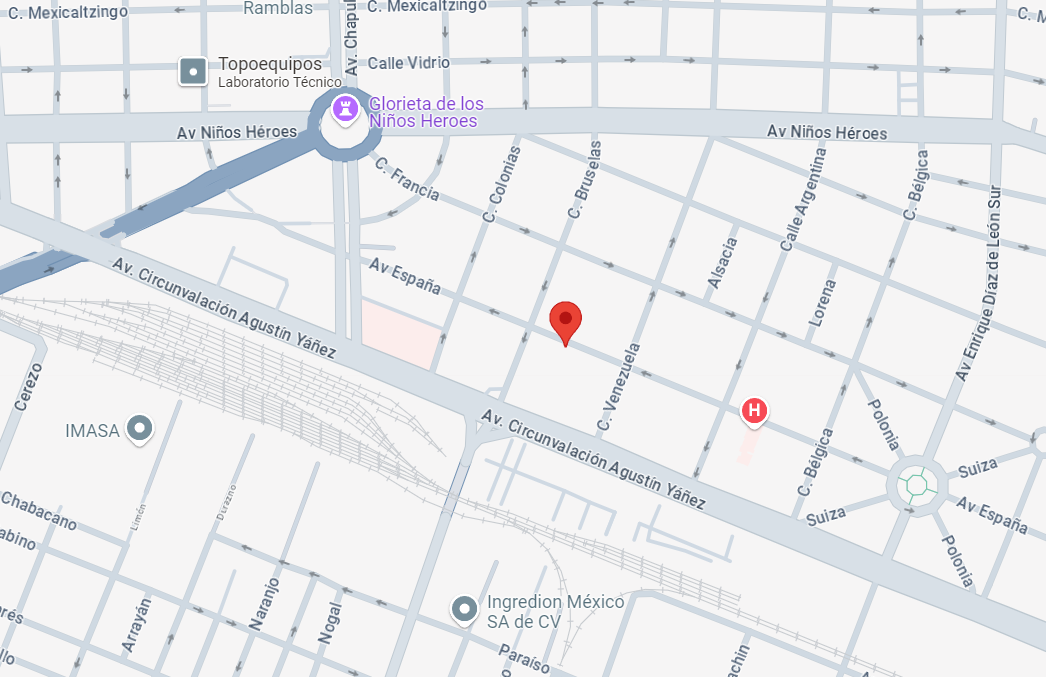
\includegraphics[width=0.8\textwidth]{Imagenes/ubicacion.png}
	\caption{Mapa ubicación Laboratoriso PiSA S.A DE C.V}\label{a1}
\end{figure}


% Poner la direcci�n y un mapa que puede salir de maps.google.com


\section{Misión}
Somos un Grupo de Empresas Responsables, confiables, éticas, con vocación de servicio; comprometidas con sus colaboradores y la salud.

\section{Visión}
Permanencia a través de innovación y crecimiento acelerado en México y en el extranjero.
	
\section{Organigrama}

\begin{figure}[H]
	\centering
	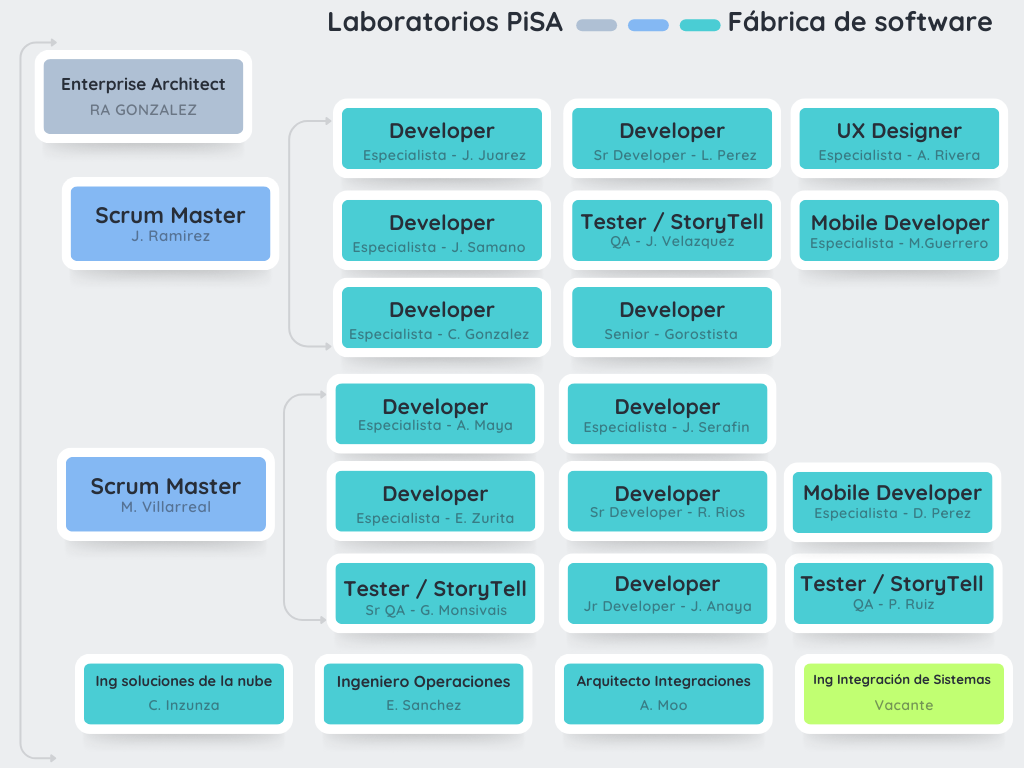
\includegraphics[width=0.9\textwidth]{Imagenes/OrganigramaPisa.png}
	\caption{Organigrama de Fábrica de Software}\label{a1}
\end{figure}
	
\section{Giro de la empresa}

PiSA Farmacéutica es una empresa dedicada a la fabricación, comercialización y distribución de medicamentos y dispositivos médicos en el tratamiento de un amplio ramo de la salud

\section{Historia}

Pisa es una empresa farmacéutica de origen mexicana que surge en el año de 1945 por iniciativa del fundador, el Profesor Don Miguel Álvarez Ochoa, quien con la valiosa colaboración de importantes profesionales de la salud, crea Productos Infantiles S. A. en respuesta a la necesidad de aquella época: contar con medicamentos especialmente diseñados y formulados para la población infantil.\\

En Productos Infantiles se comenzó a producir más de diez medicamentos diferentes, principalmente para niños: INFRAFEN, gotas para tratar los cólicos de los bebés. INFALGINA, gotas analgésicas y antipiréticas, INFANEUMIL, jarabe contra la tos, etc. los cuales fueron muy bien aceptados.\\

Todo era supervisado personalmente por el Profesor Alvarez Ochoa: desde la adquisición de materias primas y materiales para la fabricación de los productos hasta su distribución, promoción y venta.\\ 

Dada su preparación académica previa y su experiencia práctica en actividades relacionadas con la industria farmacéutica de México, era de esperar que estableciera la calidad como la primera y más estricta condición para la elaboración de los productos, una de sus responsabilidades directas.\\

El gran esfuerzo, trabajo y conocimientos de quienes conformaban en aquellos tiempos la empresa PRODUCTOS INFANTILES S.A., se vieron reflejados en su crecimiento; un crecimiento sólido que obligó al cambio y que vio cosechados sus frutos diez años después, al transformarse en LABORATORIOS PISA S.A. DE C.V.\\  

Casi 70 años después y con más de 14,000 empleados en Pisa Farmacéutica nos hemos consolidado como la empresa farmacéutica mexicana líder gracias al prestigio y a la confianza de los médicos, enfermeras, instituciones y pacientes; Elaborando productos de la más alta calidad, cumpliendo con todas las normas nacionales e internacionales que regulan la producción farmacéutica, manteniendo siempre un espíritu joven de constante innovación, mejora y crecimiento.\\

\newpage
% -------------------------------- CAPITULO PROBLEM�TICA --------------------------------------
%____________________________________________________________________________________________________________________
	
\chapter{Problemática y Descripción del Proyecto}
\newpage

% En esta secci�n se deber� redactar un planteamiento de la problem�tica que se pretende resolver.
\section{Problemática}

	En el desarrollo de software, una administración de proyectos eficiente es clave para garantizar calidad y cumplimiento de objetivos. Sin embargo, la falta de documentación técnica bien estructurada dificulta la comprensión del proyecto y afecta el trabajo de equipo, provocando así que la documentación sea inconsistente, incompleta o desactualizada, lo que dificulta la aplicación de pruebas precisas y la identificación temprana de errores.  \\
	
	La ausencia de una documentación clara y bien definida genera problemas en la comunicación entre los diferentes equipos de trabajo, dificultando la alineación de objetivos y la comprensión de los requerimientos del sistema. Esto impacta negativamente en la calidad del producto final, ya que se incrementan los riesgos de malinterpretaciones, modificaciones no documentadas y errores en la implementación.
	

%Escribir un resumen de su proyecto en donde se hable del aspecto económico, operativo, técnico, humano, objetivos, etc.
\section{Descripción del Proyecto}
	
	Desarrollar un enfoque estructurado para la elaboración de documentación técnica en proyectos de software, asegurando que sirva como una herramienta clave para la administración eficiente del desarrollo. Esta documentación permitirá mejorar la comunicación entre los equipos, optimizar la gestión de requisitos y garantizar que el software cumpla con los estándares de calidad y las expectativas del usuario final.


%Describir cual es el objetivo general que persigue el proyecto.
\subsection{Objetivo General}

	Se enfocará en la creación de guías, plantillas y metodologías que permitan documentar de manera clara los requerimientos, la arquitectura y los criterios de aceptación del software. Se trabajará en conjunto con el equipo de Quality Assurance (QA) para garantizar que la documentación cumpla con los estándares de calidad necesarios para la ejecución eficiente de pruebas y validaciones.\\
	
	Reduciendo el riesgo de errores y mejorando la trazabilidad del proyecto. Con ello, se busca optimizar la administración del proyecto, reducir tiempos de desarrollo y asegurar que el producto final cumpla con las expectativas del usuario y los estándares de la industria.\\
	
	Esta documentación facilitará la comprensión del sistema, mejorará la comunicación entre equipos y permitirá una mejor gestión de cambios, optimizando el proceso de desarrollo.
	


%Describir cuales son los objetivos específicos que persigue el proyecto. Mínimo deben ser dos y estos deben abonar al objetivo general
\subsection{Objetivos Específicos}

	1. Establecer lineamientos para la estructuración de documentos que faciliten la gestión de requisitos y planificación del desarrollo.\\
	
	2. Mejorar la comunicación entre los equipos de trabajo mediante documentación clara y organizada.\\
	
	3. Reducir el riesgo de errores en el desarrollo a través de documentación detallada y bien estructurada.\\
	
	4. Garantizar que la documentación técnica cumpla con estándares de calidad y facilite la trazabilidad del proyecto.\\
	
	5. Apoyar al equipo de Quality Assurance (QA) en la elaboración de documentación que permita validar el cumplimiento de los requisitos del software.\\

	
	
%Describir de manera detallada las actividades para el desarrollo de la estadía y/o proyecto (Diagrama de Gantt).
\subsection{Planeación}



%CAPITULO MARCO TEÓRICO: bases teorícas del proyecto. conceptos básicos y antecedentes o información existente.
%____________________________________________________________________________________________________________________
	
\chapter{Marco Teórico}
\newpage

La administración de proyectos de software es un proceso que integra metodologías y técnicas para la planificación, programación, ejecución y seguimiento de proyectos de desarrollo. Su principal objetivo es optimizar el trabajo de los desarrolladores mediante una adecuada gestión de recursos, garantizando que el proyecto se lleve a cabo de manera eficiente y productiva. Además, permite minimizar los riesgos asociados y responder de manera efectiva ante cualquier dificultad que pueda surgir en el proceso de desarrollo (Tiffin University, 2024). \\

Dentro de la administración de proyectos, la planificación juega un papel fundamental, ya que define el rumbo del proyecto desde su concepción hasta su finalización. En esta fase, se establecen los alcances, se asignan los recursos necesarios, se diseña un cronograma de ejecución y se implementan estrategias de comunicación. Asimismo, se consideran elementos clave como las pruebas y el mantenimiento del software, garantizando su correcto funcionamiento y su sostenibilidad a lo largo del tiempo (Wrike, 2024).\\

Otro aspecto esencial en el desarrollo de software es la documentación, pues permite estructurar y registrar la información clave del proyecto. A pesar de su importancia, en muchas ocasiones es percibida como una tarea que resta tiempo productivo. Sin embargo, la ausencia de documentación adecuada puede dificultar la comprensión del sistema, limitar su escalabilidad y complicar su mantenimiento a largo plazo. La documentación puede incluir especificaciones funcionales, diagramas de casos de uso y mockups de interfaces, entre otros elementos que faciliten el desarrollo y la futura gestión del software (Arsys, 2024).\\

La gestión de requisitos es otro pilar clave en la administración de proyectos de software, ya que permite definir, analizar, priorizar y validar las necesidades del sistema. Para ello, se elabora un Plan de Gestión de Requisitos (RMP), el cual establece los procesos de recopilación, documentación y control de requisitos a lo largo del ciclo de vida del proyecto. Este enfoque permite garantizar que el producto final cumpla con las expectativas del cliente y los estándares de calidad, al tiempo que facilita la detección temprana de errores y contribuye a la reducción de costos y riesgos (IBM, 2024).\\

Además de la planificación y gestión de requisitos, el Análisis de Puntos de Función (FPA, por sus siglas en inglés) se ha convertido en una herramienta fundamental en la medición de la funcionalidad de un sistema de software. Este enfoque permite cuantificar el tamaño de un proyecto con base en elementos como datos procesados, tipos de transacciones y consultas realizadas. A partir de esta información, los desarrolladores pueden identificar áreas que requieren optimización y realizar análisis comparativos de rendimiento con relación a estándares de la industria (BlueOptima, 2024).\\

El FPA también resulta útil para estimar el tiempo y los recursos necesarios en el desarrollo de un proyecto, lo que facilita una planificación más precisa y una gestión más eficiente del proceso. Su aplicación permite evaluar la productividad del equipo, monitorear el progreso del proyecto y mejorar el análisis de costo-beneficio, asegurando que las decisiones sobre inversiones y asignación de recursos se tomen de manera fundamentada. Además, contribuye a alinear los esfuerzos de desarrollo con los objetivos estratégicos de la organización, garantizando que el software desarrollado genere valor a los usuarios finales (GeeksForGeeks, 2024).\\


Las pruebas de software son un proceso esencial en el desarrollo de aplicaciones, cuyo objetivo principal es evaluar su funcionalidad e identificar posibles errores antes de su implementación final. Según Certus (2022), << este proceso garantiza que el software cumpla con los estándares de calidad y que el producto entregado sea confiable y eficiente>>.\\

En la industria del software, el aseguramiento de calidad (QA) y las pruebas forman una parte crucial del ciclo de vida del desarrollo de software (SDLC). IBM (2023) señala que defectos en el software pueden dañar la reputación de una empresa, frustrar a los clientes e incluso generar pérdidas económicas significativas. Por ello, el control de calidad es indispensable para evitar retrasos en las entregas y garantizar el funcionamiento óptico de los sistemas.\\

El control de calidad en el desarrollo de software se implementa a través de un procedimiento metódico que supervisa y revisa cada etapa del desarrollo. BrowerStack (2023) destaca que este proceso incluye actividades como análisis de requisitos, preparación de pruebas, ejecución de pruebas, seguimiento de defectos y redacción de informes.\\

IBM (2023) resalta que la tendencia actual en la industria es realizar pruebas continuas, es decir, iniciar las pruebas desde la fase de diseño, continuar con ellas durante el desarrollo y mantenerlas incluso en producción. Este enfoque permite detectar errores con mayor anticipación y mejorar la calidad del producto final.\\

Para logar una validación integral del software, es fundamental definir correctamente los escenarios y casos de prueba. Leapwork (2025) los describe de la siguiente manera
Los escenarios de prueba es un documento de alto nivel que describe la funcionalidad que se evaluará, proporcionando una visión general de lo que debe probarse. Se centra en el comportamiento de software sin entrar en detalles específicos.\\

Los casos de prueba son un conjunto de condiciones o variables específicas que permiten evaluar si un sistema cumple con los requisitos establecidos. Incluyendo entradas, condiciones, procedimiento y resultados esperado, guiando al evaluador paso a paso.\\

La correcta implementación de estos elementos permite asegurar el correcto funcionamiento del software en diversas situaciones y garantizar un producto de alta calidad. Como afirma IBM (2023), las pruebas continuas y bien estructuradas contribuyen a minimizar riesgos y mejorar la satisfacción del usuario final, optimizando el rendimiento de las aplicaciones en un mercado altamente competitivo.\\




%CAPITULO DESARROLLO DEL PROYECTO: procedimiento o descripci�n de las actividades realizadas, como es un desarrollo es importante
%____________________________________________________________________________________________________________________


\chapter{Desarrollo del Proyecto}
\newpage
	
\section{Path de ayuda}

	El proyecto Path de Ayuda está diseñado para mejorar la eficiencia en la planta de Formas Sólidas, proporcionando un sistema de monitoreo en tiempo real que facilite la gestión del proceso de fabricación. Este sistema permitirá visualizar el avance de los lotes en cada línea de producción, agilizar la planificación de cambios y limpiezas, así como gestionar alertas sobre posibles fallas, notificando a los dispositivos vinculados del personal responsable.\\
	
	Se participó en la fase inicial del proyecto, enfocándose en la documentación necesaria para su desarrollo. Dado que la implementación del sistema sería realizada por una empresa externa, nuestra labor consistió en estructurar la información clave, garantizar una base organizada y clara para su desarrollo.\\
	
	Se logró una mejor organización del proyecto, facilitando la transición hacia el equipo de desarrollo externo y asegurando que las necesidades del negocio fueran correctamente traducidas en especificaciones técnicas.

\subsection{Levantamiento de requerimeintos}

	Para garantizar que el proyecto Path de Ayuda cumpliera con las necesidades operativas de la planta de Formas Sólidas, llevamos a cabo un proceso de levantamiento de requerimientos con el objetivo de documentar de manera precisa las funcionalidades y características esenciales del sistema.\\
	
	Durante este proceso, uno de los mayores desafíos fue traducir las necesidades operativas en especificaciones técnicas claras, asegurando que el sistema cumpliera con los estándares requeridos.\\
	
	Gracias a este levantamiento de información, el equipo de desarrollo externo pudo contar con una documentación estructurada y detallada, facilitando la implementación del sistema y asegurando que el producto final estuviera alineado con los objetivos de la organización.

\subsection{Descripción de Épicas}

	Como parte de la documentación para el desarrollo del sistema Path de Ayuda, se realizó la definición y estructuración de las épicas del proyecto. Una épica representa un conjunto de funcionalidades de alto nivel que permiten organizar el trabajo en historias de usuario más detalladas, facilitando la planificación del desarrollo.\\
	
	Para garantizar una documentación clara y estandarizada, cada épica fue documentada en un formato estructurado de la siguiente manera:\\
		
	{\leftskip=1em 
		\noindent 
		1. Título de la Épica – Nombre que resume su propósito.
	\par}
	
	{\leftskip=1em 
		\noindent 
		2. Descripción – Explicación detallada de la funcionalidad y su importancia.
	\par}
	
	{\leftskip=1em 
		\noindent 
		3. Criterios de Aceptación – Reglas y condiciones necesarias para que la épica se considere completada.\\
	\par}

	El equipo de QA desempeñó un rol clave en la validación de cada épica, asegurando que la información estuviera completa y alineada con los requisitos del negocio. Gracias a esta documentación, el equipo de desarrollo externo pudo comprender mejor el alcance del proyecto, optimizando los tiempos de implementación y reduciendo posibles errores o ambigüedades en el desarrollo.
	
\subsection{Puntos de Función}

	Como parte del proceso de documentación del proyecto Path de Ayuda, se realizó un Análisis de Punto de Función (APF) para estimar el tamaño del software y evaluar el esfuerzo necesario para su desarrollo. Esta técnica permitió cuantificar las funcionalidades del sistema basándose en la perspectiva del usuario, facilitando una mejor planificación del proyecto y una estimación más precisa de costos y tiempos de desarrollo.\\
	
	Para llevar a cabo el análisis, se identificaron y clasificaron los siguientes elementos del sistema:\\
	
	{\leftskip=1em 
	  \noindent 
		1.Entradas Externas (EI) – Datos ingresados por los usuarios en el sistema.
	\par}
	
	{\leftskip=1em 
	  \noindent 
		2.Salidas Externas (EO) – Información generada y presentada a los usuarios.
	\par}
	
	{\leftskip=1em 
	  \noindent 
		3.Consultas Externas (EQ) – Procesos que permiten a los usuarios recuperar información específica
	\par}

	{\leftskip=1em 
	  \noindent 
		4.Archivos Lógicos Internos (ILF) – Bases de datos o archivos que almacenan información persistente.
	\par}

	\begin{figure}[htp]
		\centering
		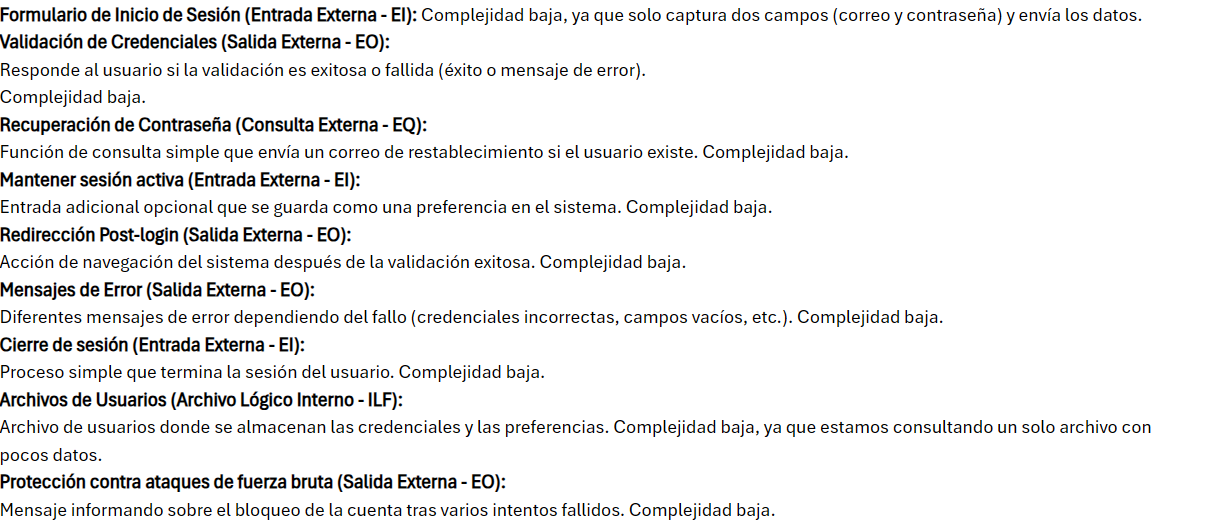
\includegraphics[width=1.0\textwidth]
		{Imagenes/PathAyuda/FpsLogin.png}
		\caption{Puntos de Función - Login}\label{a1}
	\end{figure}
	
	\begin{figure}[H]
		\centering
		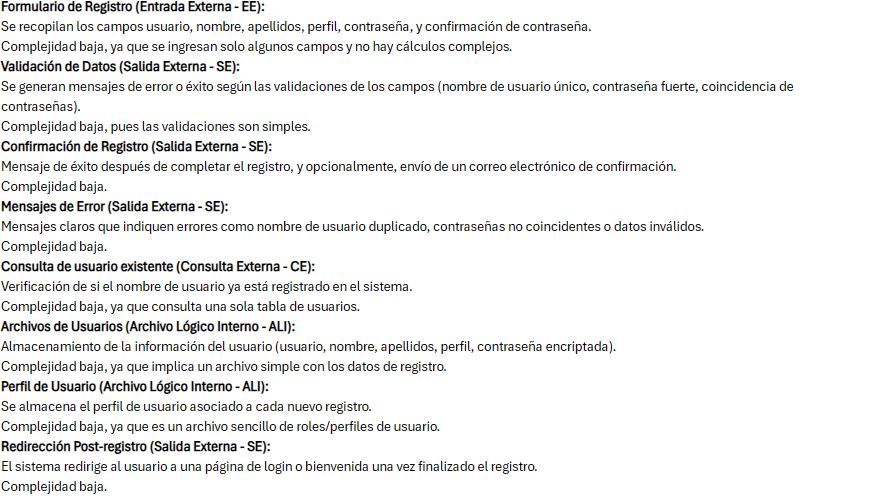
\includegraphics[width=1.0\textwidth]
		{Imagenes/PathAyuda/FpsRegistroUsuario.png}
		\caption{Puntos de Función - Registo de Usuarios}\label{a2}
	\end{figure}

	\begin{figure}[H]
		\centering
		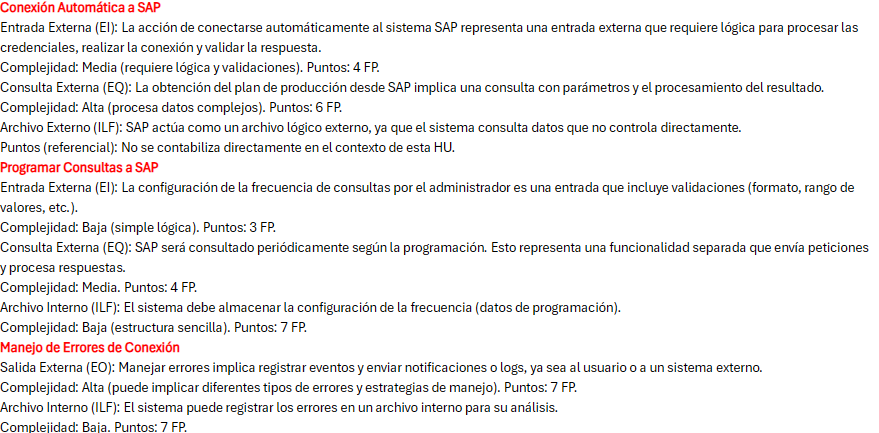
\includegraphics[width=1.0\textwidth]
		{Imagenes/PathAyuda/FpsIntegracionSAP.png}
		\caption{Puntos de Función - Integración de SAP}\label{a2}
	\end{figure}

	\begin{figure}[H]
		\centering
		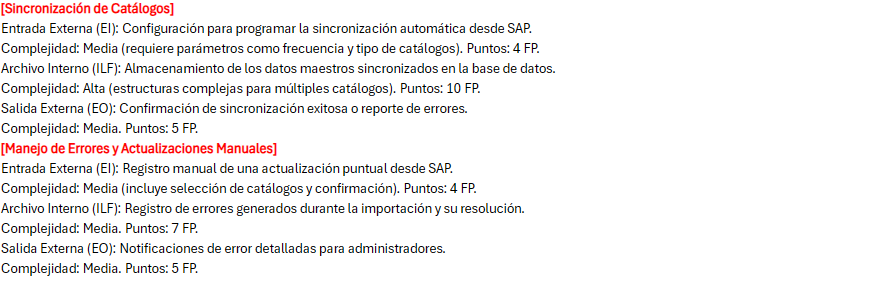
\includegraphics[width=1.0\textwidth]
		{Imagenes/PathAyuda/FpsCatalagoSAP.png}
		\caption{Puntos de Función - Catalagos SAP}\label{a2}
	\end{figure}
	
	\begin{figure}[H]
		\centering
		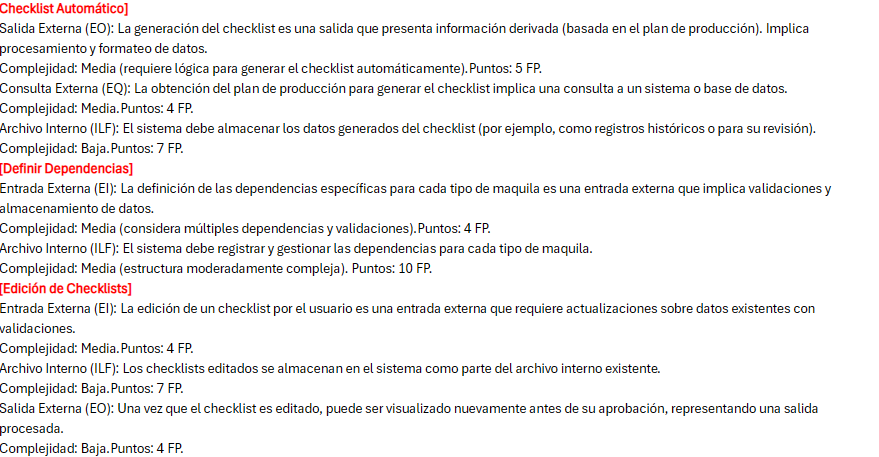
\includegraphics[width=1.0\textwidth]
		{Imagenes/PathAyuda/FpsDependeciasChecklist.png}
		\caption{Puntos de Función - Gestión de Dependencias y Checklist
		}\label{a2}
	\end{figure}
	
	\begin{figure}[H]
		\centering
		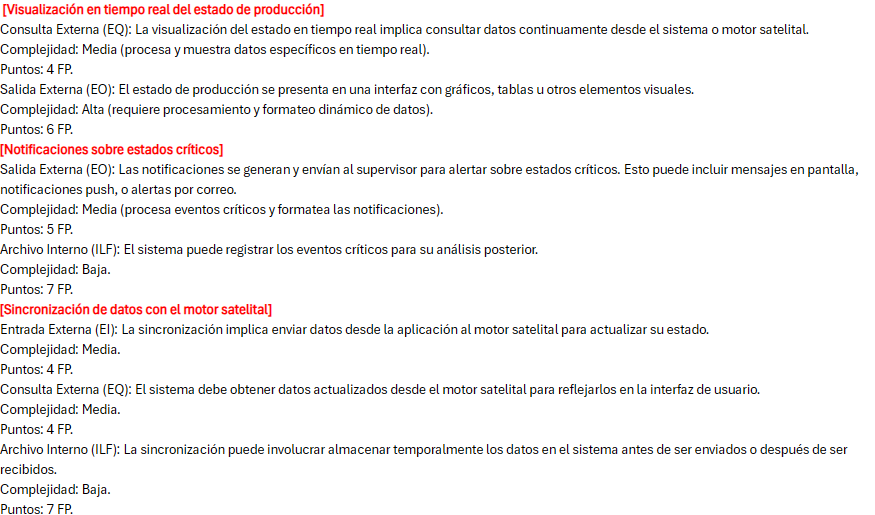
\includegraphics[width=1.0\textwidth]
		{Imagenes/PathAyuda/FpsComunicacionPiso.png}
		\caption{Puntos de Función - Comunicación con el Control de Piso 
		}\label{a2}
	\end{figure}
	
	\begin{figure}[H]
		\centering
		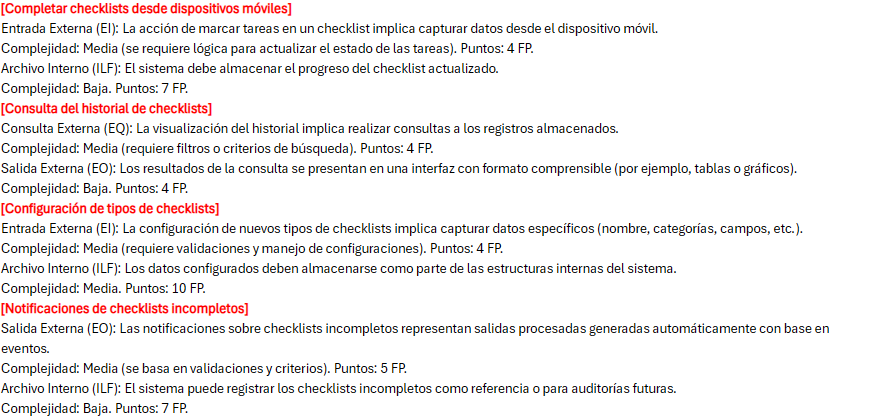
\includegraphics[width=1.0\textwidth]
		{Imagenes/PathAyuda/FpsChecklistsInteractivos.png}
		\caption{Puntos de Función - Gestión de Checklists Interactivos 
		}\label{a2}
	\end{figure}
	
	\begin{figure}[H]
		\centering
		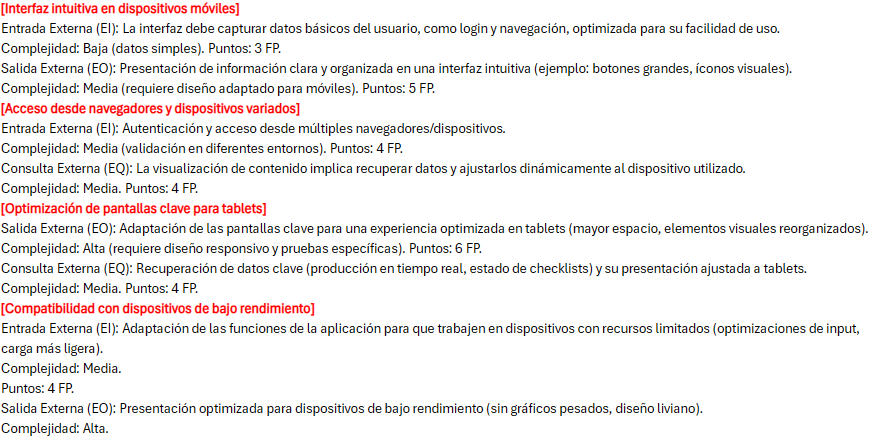
\includegraphics[width=1.0\textwidth]
		{Imagenes/PathAyuda/FpsInterfacesUsuario.png}
		\caption{Puntos de Función - Desarrollo de Interfaces de Usuario Adaptativas 
		}\label{a2}
	\end{figure}
	
	\begin{figure}[H]
		\centering
		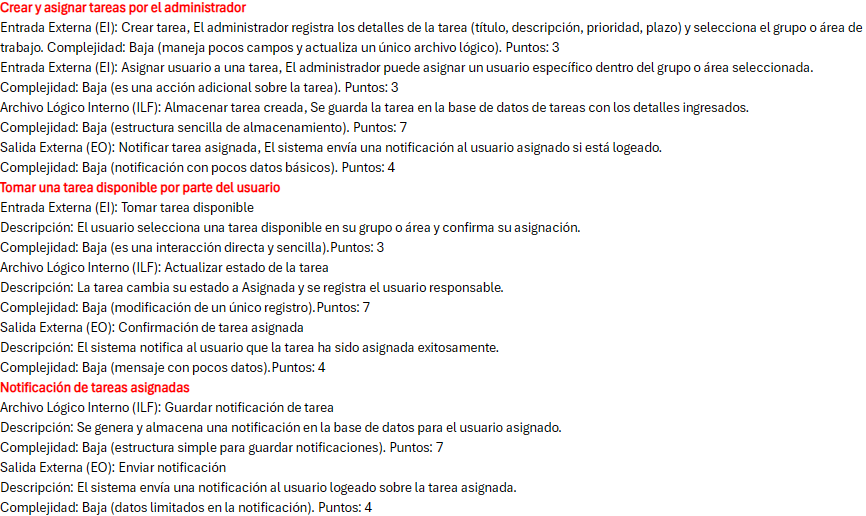
\includegraphics[width=1.0\textwidth]
		{Imagenes/PathAyuda/FpsTaskmanager.png}
		\caption{Puntos de Función - Task manager 
		}\label{a2}
	\end{figure}
	
	\begin{figure}[H]
		\centering
		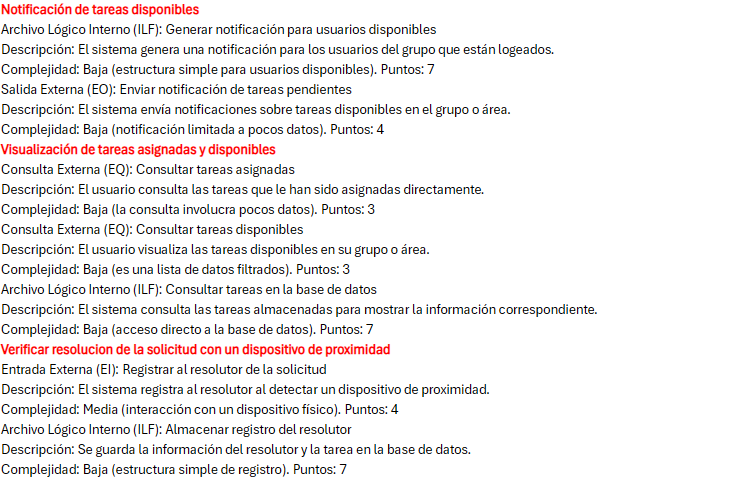
\includegraphics[width=1.0\textwidth]
		{Imagenes/PathAyuda/FpsTaskmanager2.png}
		\caption{Puntos de Función - Task manager 
		}\label{a2}
	\end{figure}
	
	\begin{figure}[H]
		\centering
		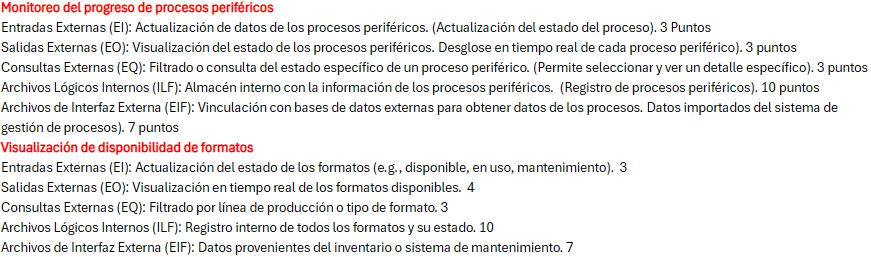
\includegraphics[width=1.0\textwidth]
		{Imagenes/PathAyuda/FpsSMED.png}
		\caption{Puntos de Función - SMED
		}\label{a2}
	\end{figure}
	
	\begin{figure}[H]
		\centering
		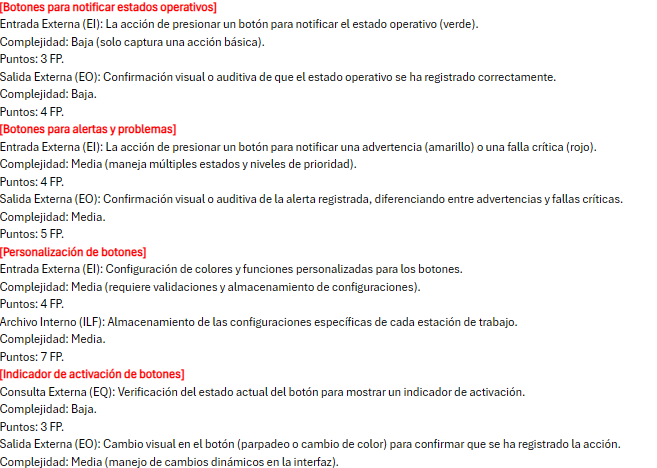
\includegraphics[width=1.0\textwidth]
		{Imagenes/PathAyuda/FpsBotonesANDON.png}
		\caption{Puntos de Función - Simulación de Botones del Sistema ANDON 
		}\label{a2}
	\end{figure}

	
	\begin{figure}[H]
		\centering
		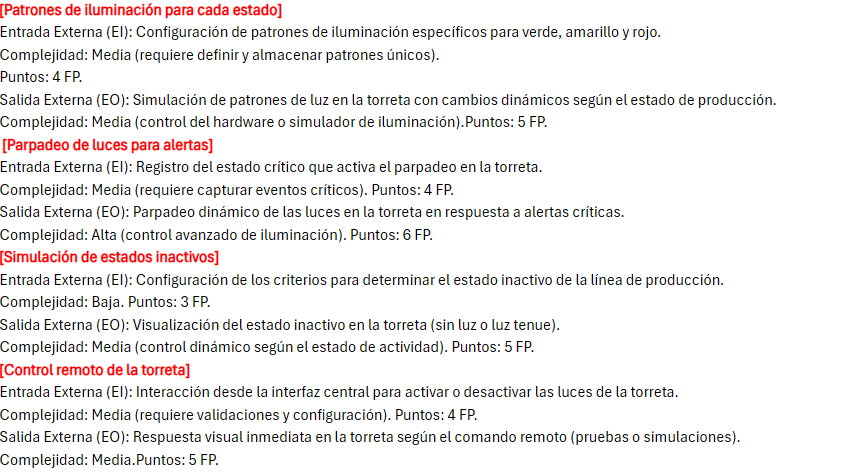
\includegraphics[width=1.0\textwidth]
		{Imagenes/PathAyuda/FpsTorretasLuminosas.png}
		\caption{Puntos de Función - Configuración y Simulación de Torretas Luminosas  
		}\label{a2}
	\end{figure}
	
	\begin{figure}[H]
		\centering
		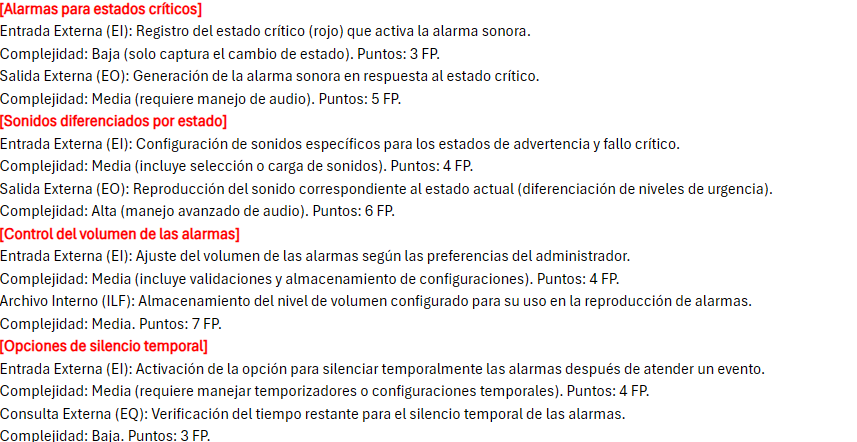
\includegraphics[width=1.0\textwidth]
		{Imagenes/PathAyuda/FpsAlarmasNotifiaciones.png}
		\caption{Puntos de Función - Implementación de Alarmas y Notificaciones Auditivas 
		}\label{a2}
	\end{figure}
	
	\begin{figure}[H]
		\centering
		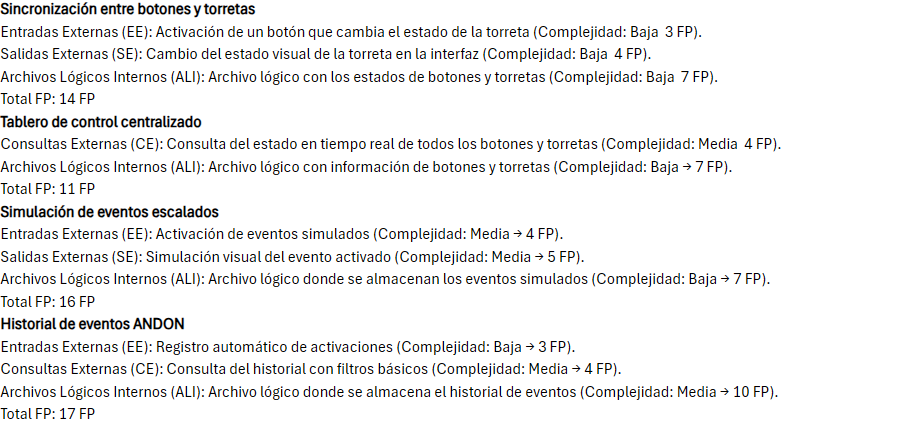
\includegraphics[width=1.0\textwidth]
		{Imagenes/PathAyuda/FpsSimulacion.png}
		\caption{Puntos de Función - Integración y Simulación de la Interfaz ANDON Completa 
		}\label{a2}
	\end{figure}
	
	\begin{figure}[H]
		\centering
		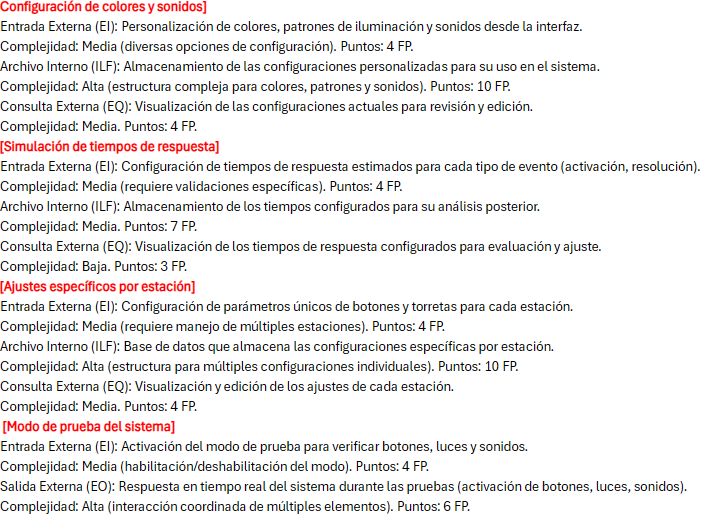
\includegraphics[width=1.0\textwidth]
		{Imagenes/PathAyuda/FpsPersonalizacionAndon.png}
		\caption{Puntos de Función - Personalización y Configuración del Sistema ANDON
		}\label{a2}
	\end{figure}
	
	\begin{figure}[H]
		\centering
		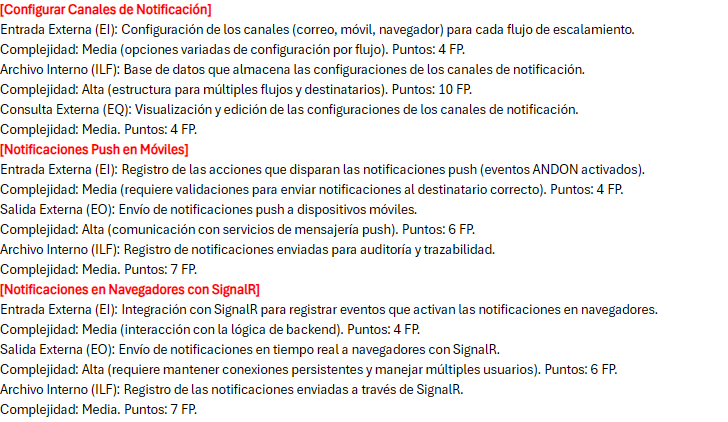
\includegraphics[width=1.0\textwidth]
		{Imagenes/PathAyuda/FpsMultiCanal.png}
		\caption{Puntos de Función - Integración de Notificaciones Multi-Canal
		}\label{a2}
	\end{figure}
	
	\begin{figure}[H]
		\centering
		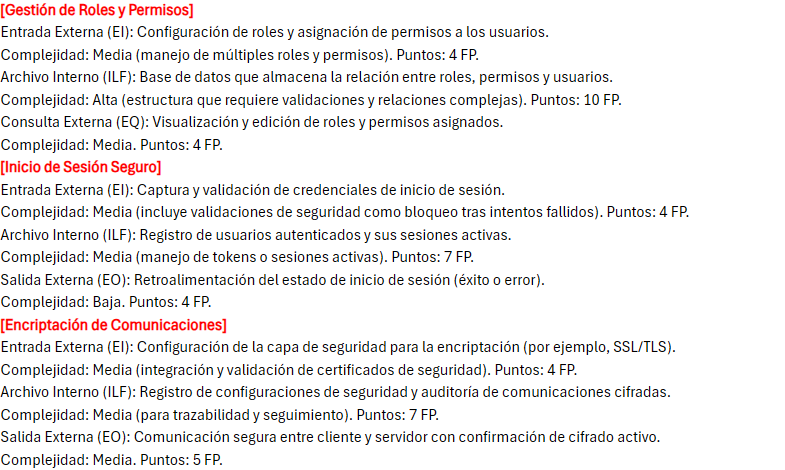
\includegraphics[width=1.0\textwidth]
		{Imagenes/PathAyuda/FpsSeguridadAutenticacion.png}
		\caption{Puntos de Función - Seguridad y Autenticación
		}\label{a2}
	\end{figure}
	
	\begin{figure}[H]
		\centering
		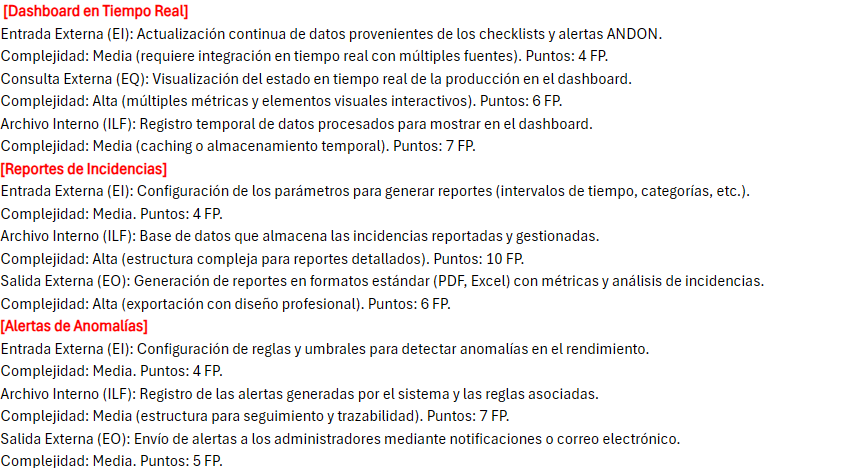
\includegraphics[width=1.0\textwidth]
		{Imagenes/PathAyuda/FpsMonitoreoReportes.png}
		\caption{Puntos de Función - Monitoreo y Reportes
		}\label{a2}
	\end{figure}
	
	\begin{figure}[H]
		\centering
		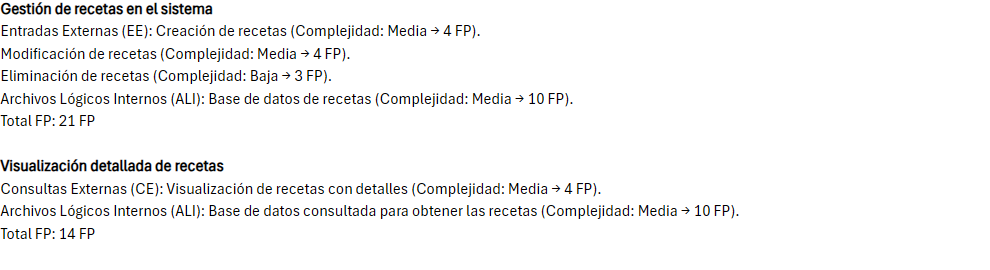
\includegraphics[width=1.0\textwidth]
		{Imagenes/PathAyuda/FpsRecetas.png}
		\caption{Puntos de Función - Recetas
		}\label{a2}
	\end{figure}
	
	\begin{figure}[H]
		\centering
		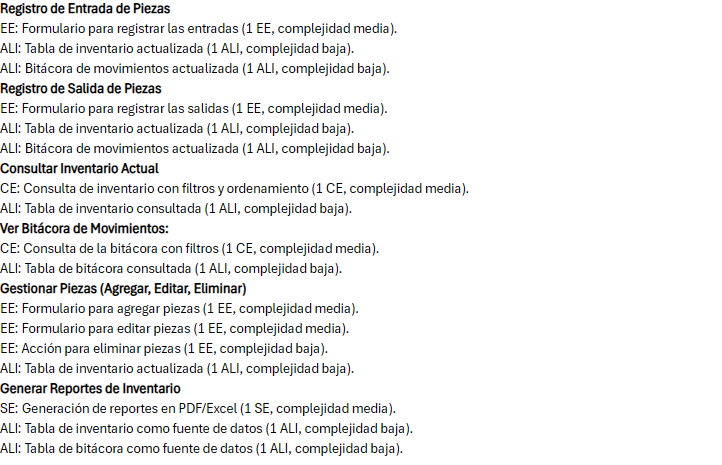
\includegraphics[width=1.0\textwidth]
		{Imagenes/PathAyuda/FpsInventarios.png}
		\caption{Puntos de Función - Inventarios
		}\label{a2}
	\end{figure}
	
	\begin{figure}[H]
		\centering
		\includegraphics[width=1.0\textwidth]
		{Imagenes/PathAyuda/FpsProgramaciónTareas.png}
		\caption{Puntos de Función - Programación de tareas 
		}\label{a2}
	\end{figure}
\newpage

\subsection{Casos de prueba}

	Como parte del proceso de aseguramiento de calidad para el sistema Path de Ayuda, se elaboró un documento estructurado de casos de prueba, organizados por épicas y sus respectivos casos de prueba.\\
	
	El propósito principal de este documento fue definir y estructurar pruebas que permitieran evaluar el cumplimiento de los requerimientos antes de la fase de desarrollo, asegurando que el sistema funcione correctamente bajo diferentes condiciones.\\
	
	El documento de casos de prueba se organizó por épicas, y dentro de cada épica se definieron los escenarios a evaluar.\\
	
	{\leftskip=1em 
	\noindent 
		\textbf{Escenario:} Situación específica en la que se ejecutará la prueba.
	\par}
	
	{\leftskip=1em 
	\noindent 
		\textbf{Prerrequisitos:} Condiciones que deben cumplirse antes de ejecutar la prueba
	\par}

	{\leftskip=1em 
	\noindent 
		\textbf{Datos de Entrada:} Información que se ingresará en el sistema para la ejecución de la prueba.
	\par}

	{\leftskip=1em 
	\noindent 
		\textbf{Resultados Esperados:} Comportamiento esperado del sistema tras ejecutar la prueba.
	\par}

	{\leftskip=1em 
	\noindent 
		\textbf{Escenarios Positivos:} Pruebas en las que el sistema responde correctamente según lo esperado.
	\par}

	{\leftskip=1em 
	\noindent 
		\textbf{Escenarios Negativos:} Pruebas en las que se validan errores o respuestas incorrectas del sistema.\\
	\par}
	
	\begin{figure}[H]
		\centering
		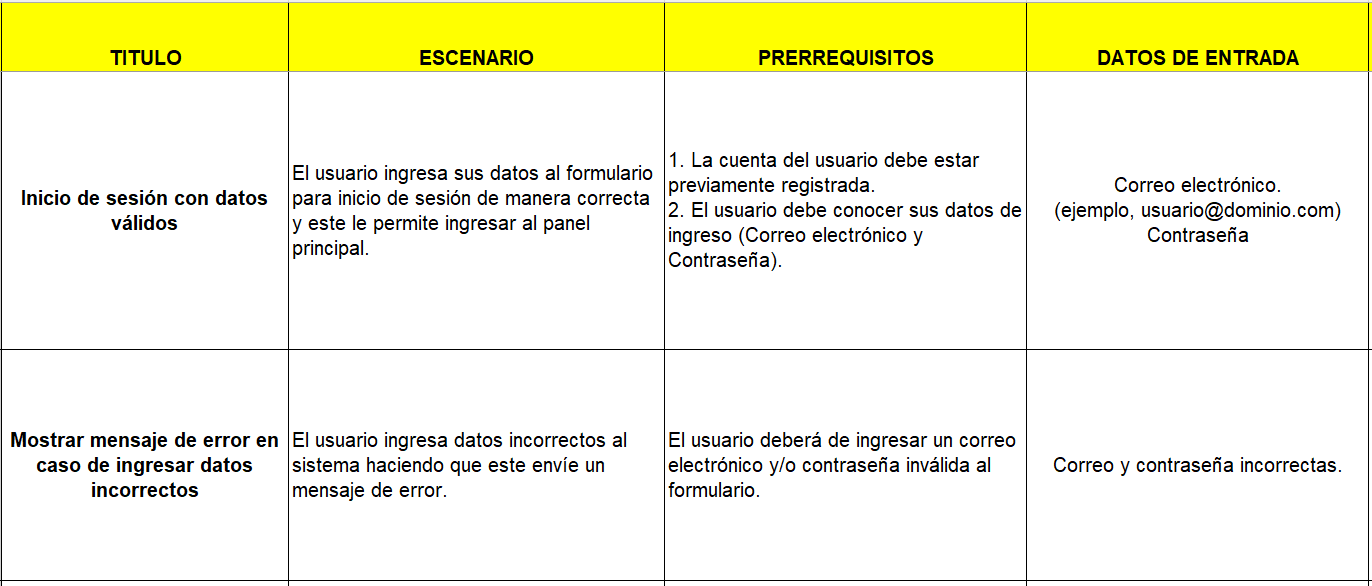
\includegraphics[width=1.0\textwidth]
		{Imagenes/PathAyuda/CPLogin.png}
		\caption{Caso de Prueba - Log-in 
		}\label{a2}
	\end{figure}
	
	\begin{figure}[H]
		\centering
		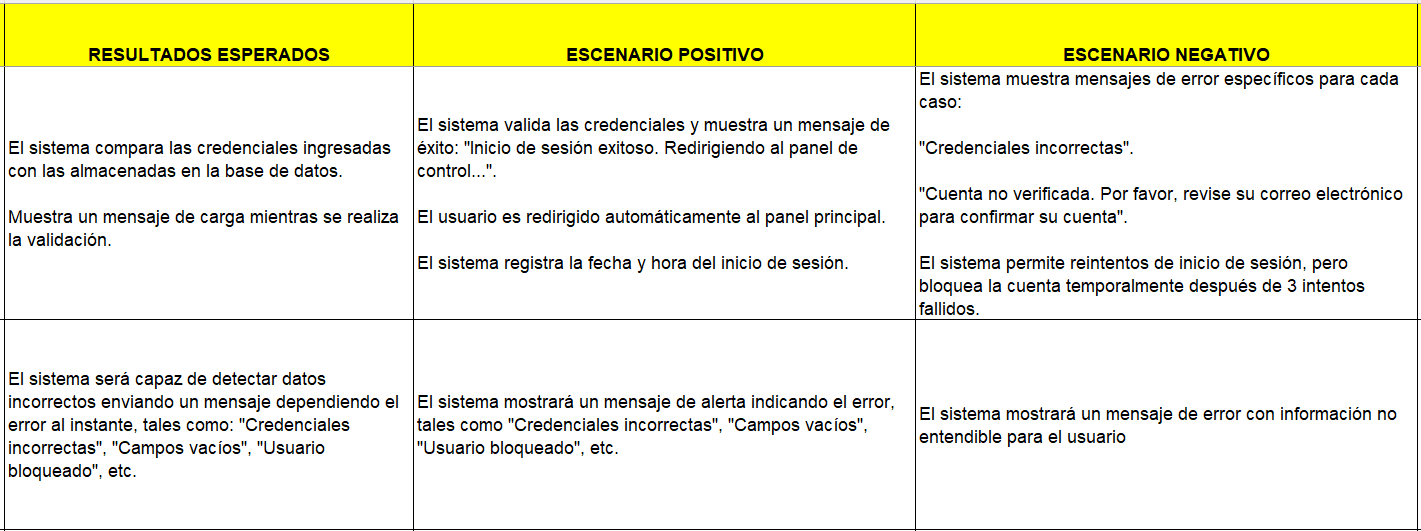
\includegraphics[width=1.0\textwidth]
		{Imagenes/PathAyuda/CPLogin2.png}
		\caption{Caso de Prueba - Log-in 
		}\label{a2}
	\end{figure}

	\begin{figure}[H]
		\centering
		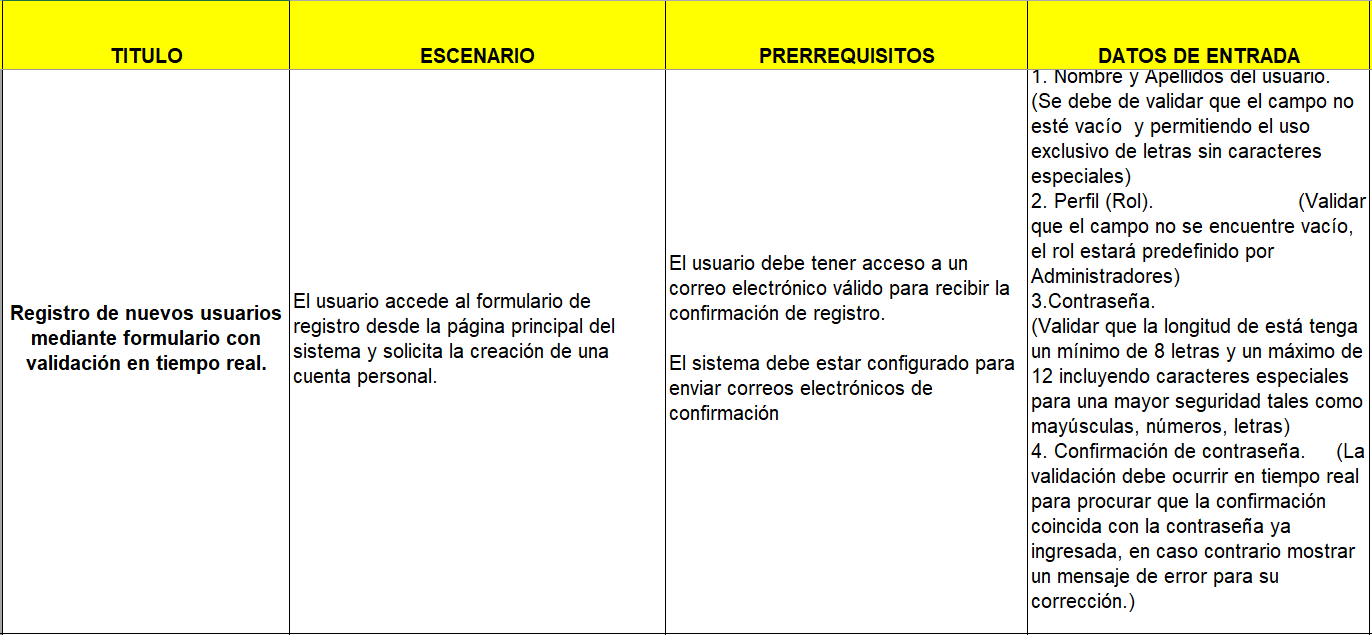
\includegraphics[width=1.0\textwidth]
		{Imagenes/PathAyuda/CPRegistroUsuario.png}
		\caption{Caso de Prueba - Registro de Usuario 
		}\label{a2}
	\end{figure}
	
	\begin{figure}[H]
		\centering
		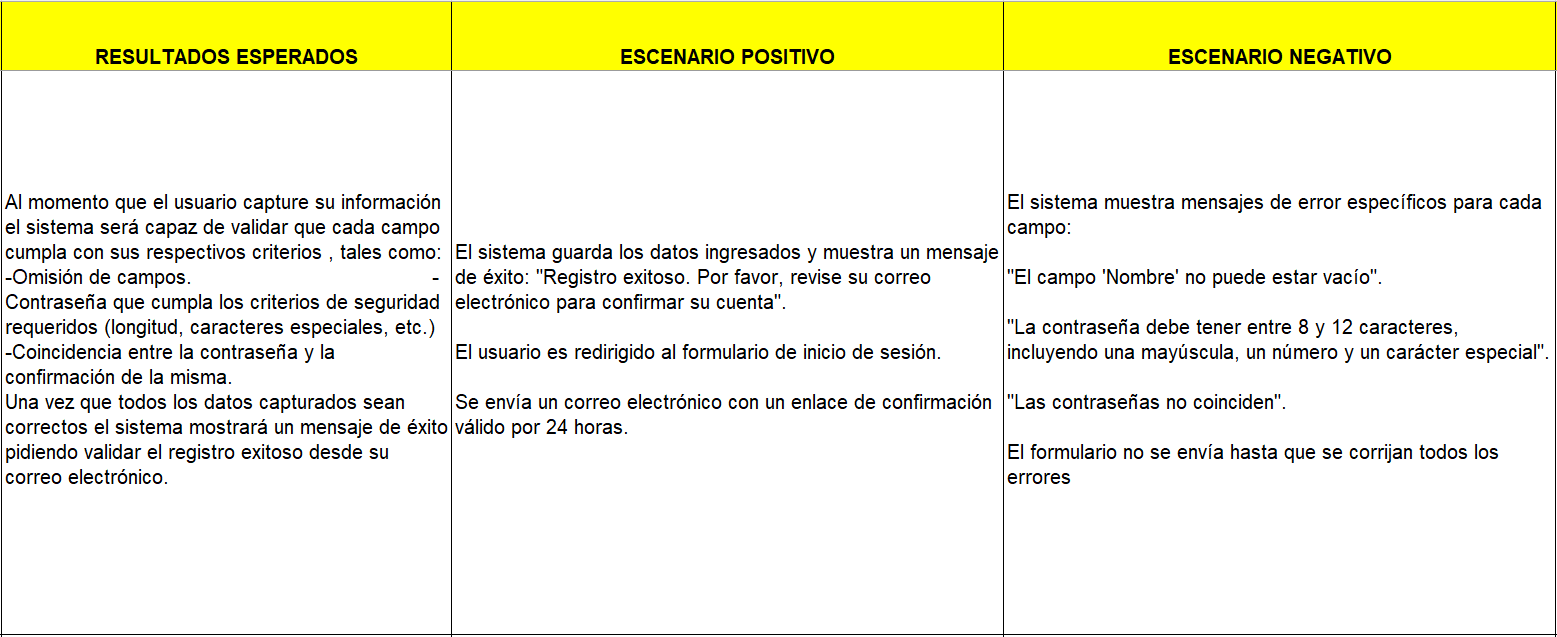
\includegraphics[width=1.0\textwidth]
		{Imagenes/PathAyuda/CPRegistroUsuario2.png}
		\caption{Caso de Prueba - Registro de Usuario
		}\label{a2}
	\end{figure}
	
	\begin{figure}[H]
		\centering
		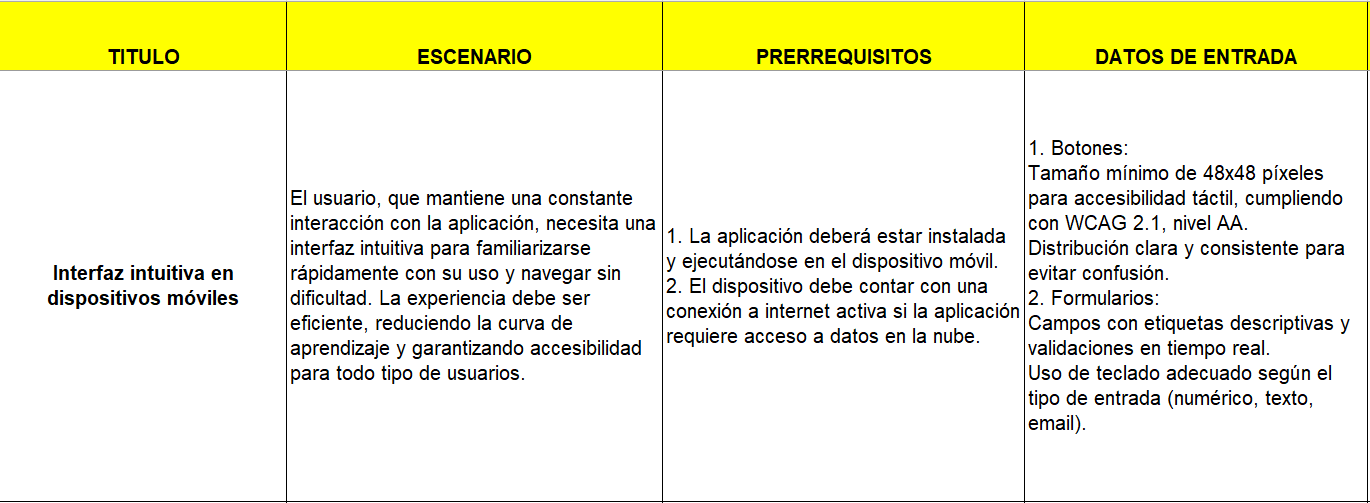
\includegraphics[width=1.0\textwidth]
		{Imagenes/PathAyuda/CPInterfaces.png}
		\caption{Caso de Prueba - Desarrollo de Interfaces de Usuario Adaptativas 
		}\label{a2}
	\end{figure}
	
	\begin{figure}[H]
		\centering
		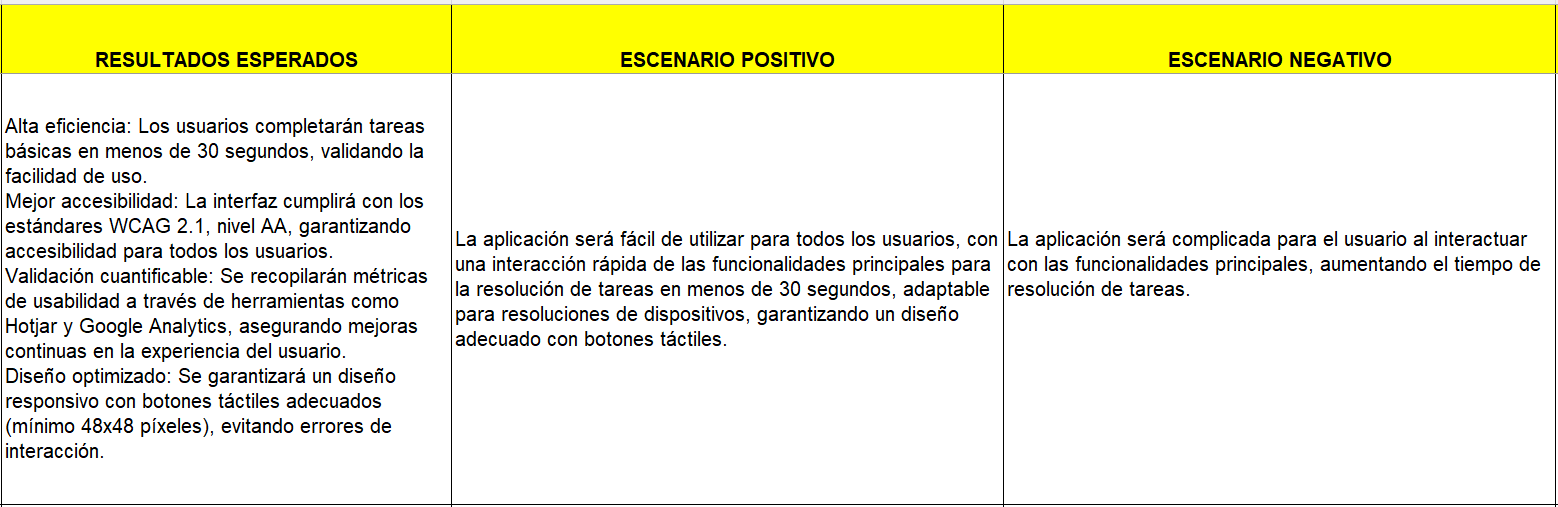
\includegraphics[width=1.0\textwidth]
		{Imagenes/PathAyuda/CPInterfaces2.png}
		\caption{Caso de Prueba - Desarrollo de Interfaces de Usuario Adaptativas
		}\label{a2}
	\end{figure}
	
	\begin{figure}[H]
		\centering
		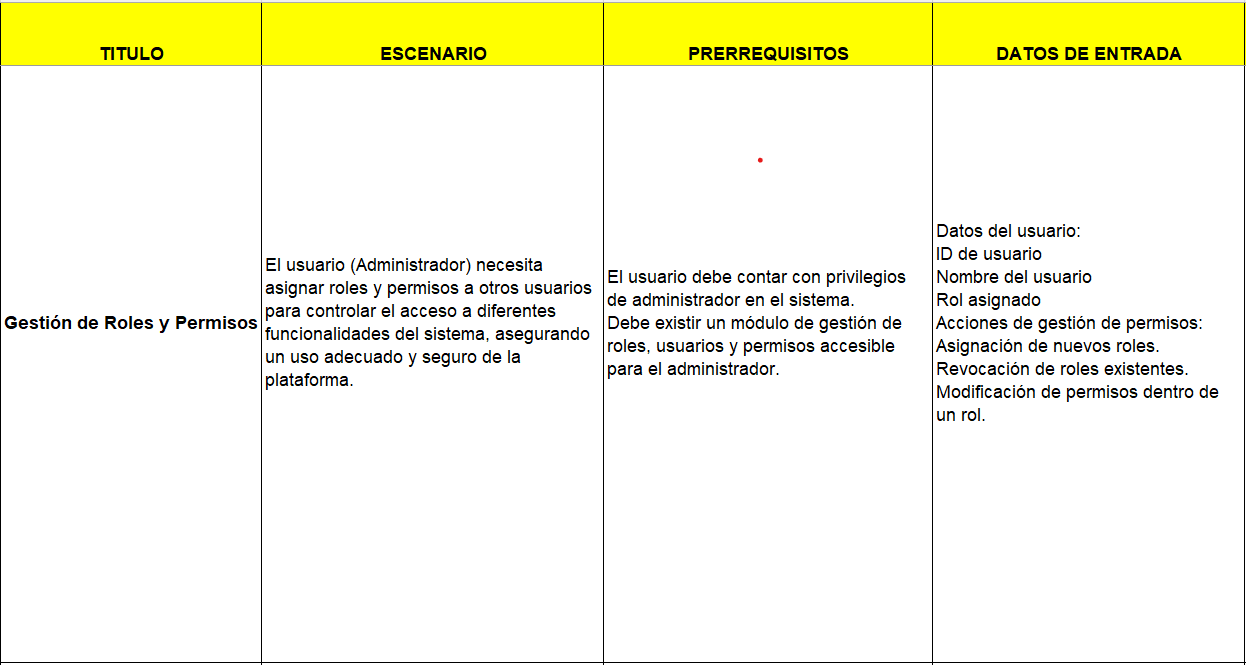
\includegraphics[width=1.0\textwidth]
		{Imagenes/PathAyuda/CPSeguridadAutenticacion.png}
		\caption{Caso de Prueba - Seguridad y  Autenticación
		}\label{a2}
	\end{figure}
	
	\begin{figure}[H]
		\centering
		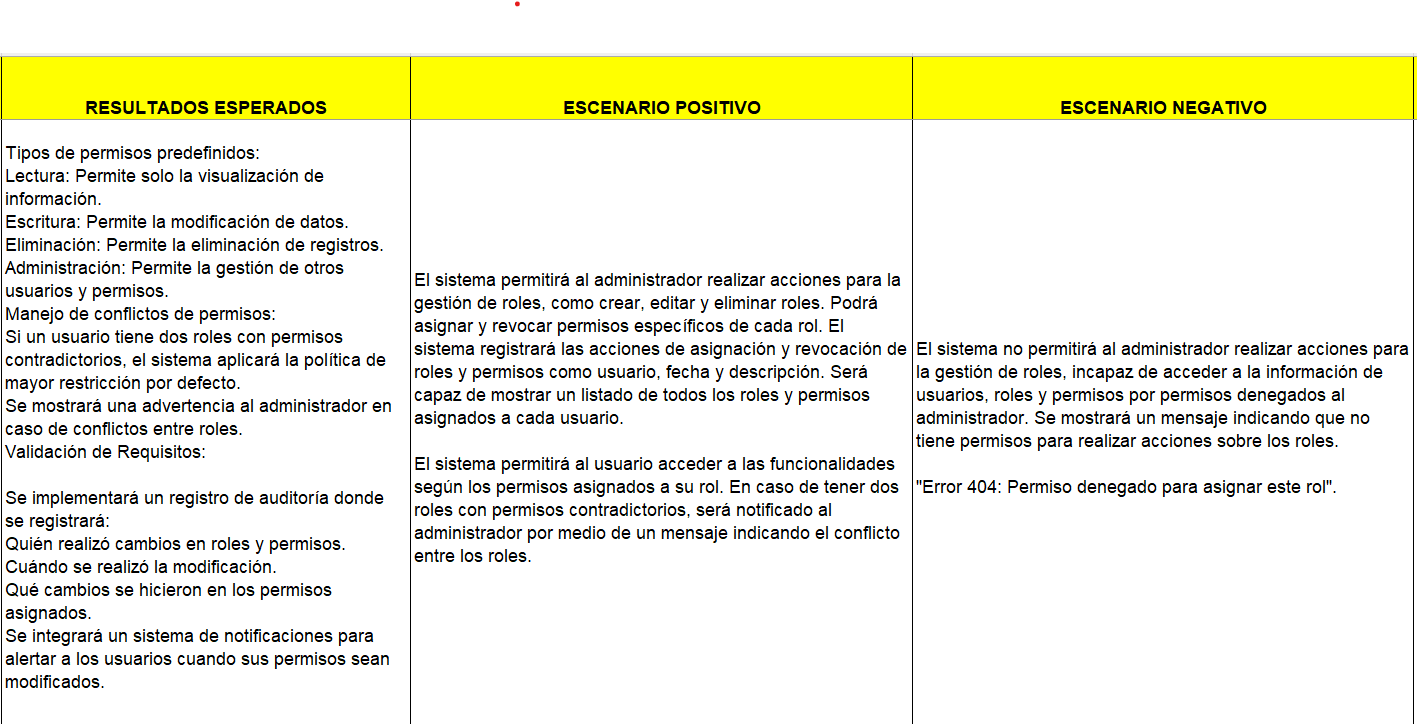
\includegraphics[width=1.0\textwidth]
		{Imagenes/PathAyuda/CPSeguridadAutenticacion2.png}
		\caption{Caso de Prueba - Seguridad y  Autenticación
		}\label{a2}
	\end{figure}
	
	\begin{figure}[H]
		\centering
		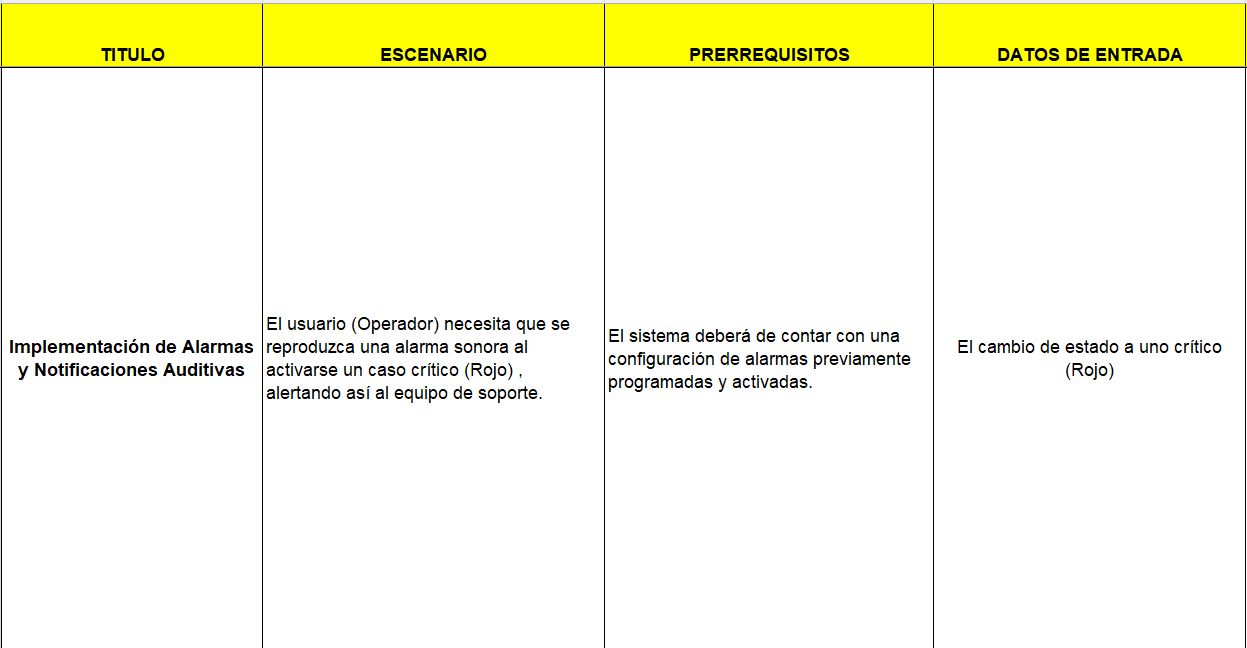
\includegraphics[width=1.0\textwidth]
		{Imagenes/PathAyuda/CPPathAyuda.png}
		\caption{Caso de Prueba - Path de ayuda /  ANDON
		}\label{a2}
	\end{figure}
	
	\begin{figure}[H]
		\centering
		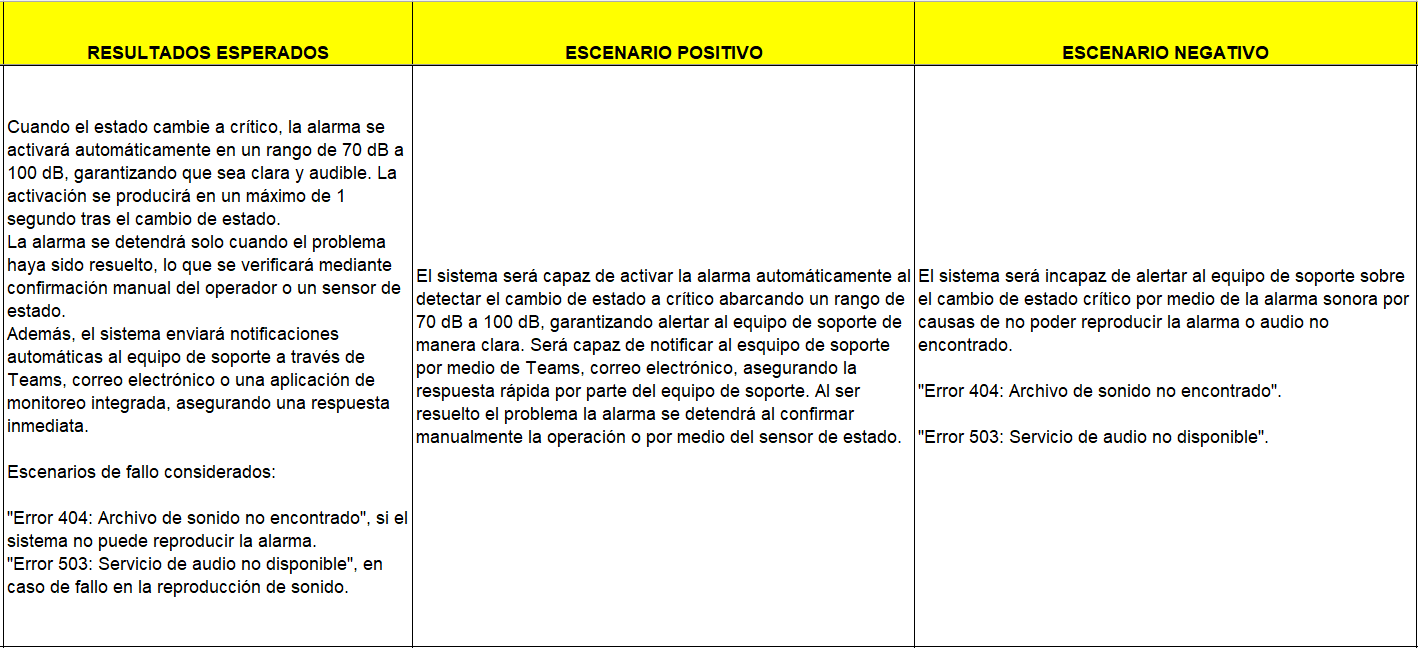
\includegraphics[width=1.0\textwidth]
		{Imagenes/PathAyuda/CPPathAyuda2.png}
		\caption{Caso de Prueba - Path de ayuda /  ANDON
		}\label{a2}
	\end{figure}
	
	\begin{figure}[H]
		\centering
		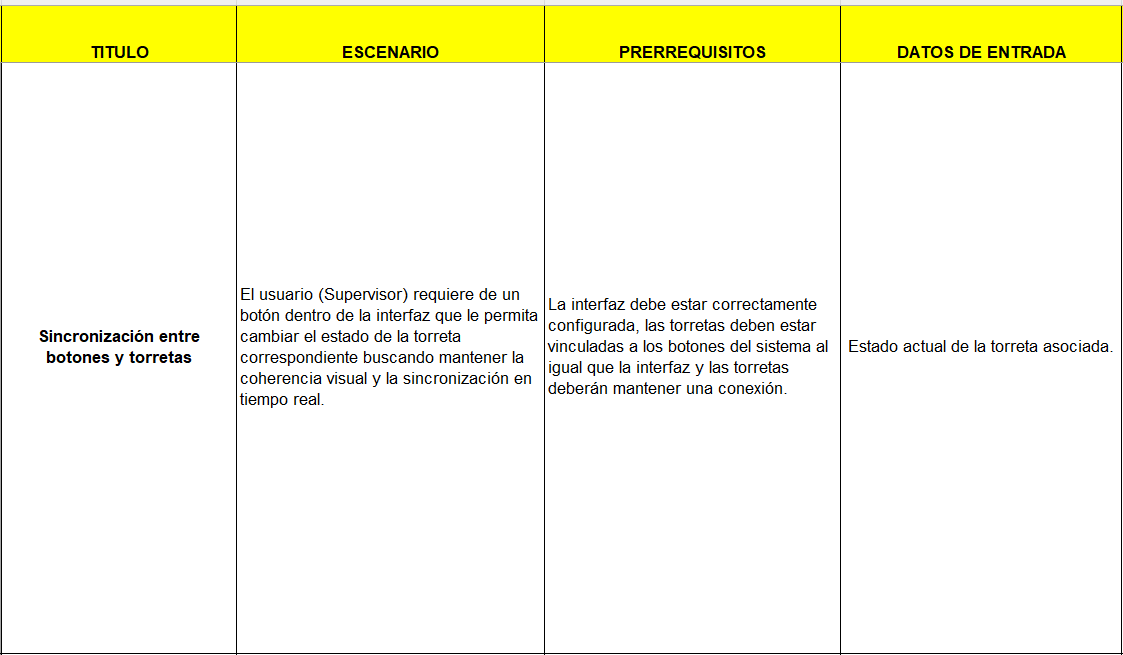
\includegraphics[width=1.0\textwidth]
		{Imagenes/PathAyuda/CPANDON.png}
		\caption{Caso de Prueba - Integración y simulación - ANDON
		}\label{a2}
	\end{figure}
	
	\begin{figure}[H]
		\centering
		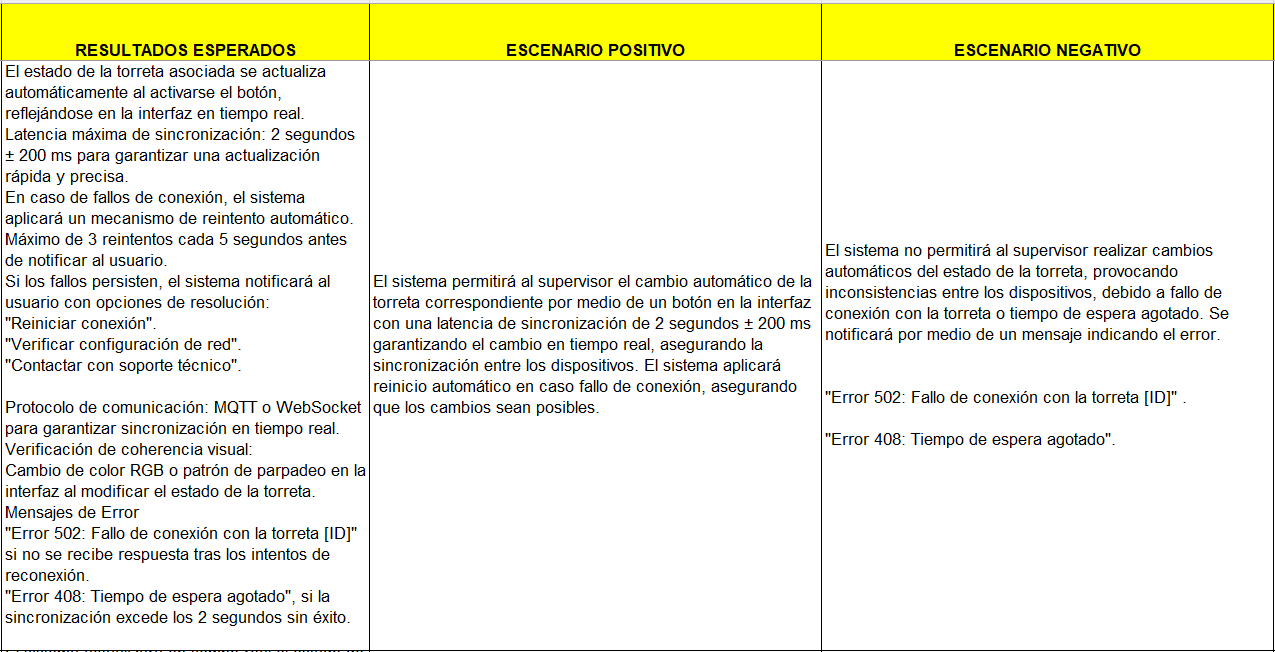
\includegraphics[width=1.0\textwidth]
		{Imagenes/PathAyuda/CPANDON2.png}
		\caption{Caso de Prueba - Integración y simulación - ANDON
		}\label{a2}
	\end{figure}
	
	\begin{figure}[H]
		\centering
		\includegraphics[width=1.0\textwidth]
		{Imagenes/PathAyuda/CPPesonalizaciónANDON.png}
		\caption{Caso de Prueba - Personalización y configuración - ANDON 
		}\label{a2}
	\end{figure}
	
	\begin{figure}[H]
		\centering
		\includegraphics[width=1.0\textwidth]
		{Imagenes/PathAyuda/CPPesonalizaciónANDON2.png}
		\caption{Caso de Prueba - Personalización y configuración - ANDON
		}\label{a2}
	\end{figure}
	
	\begin{figure}[H]
		\centering
		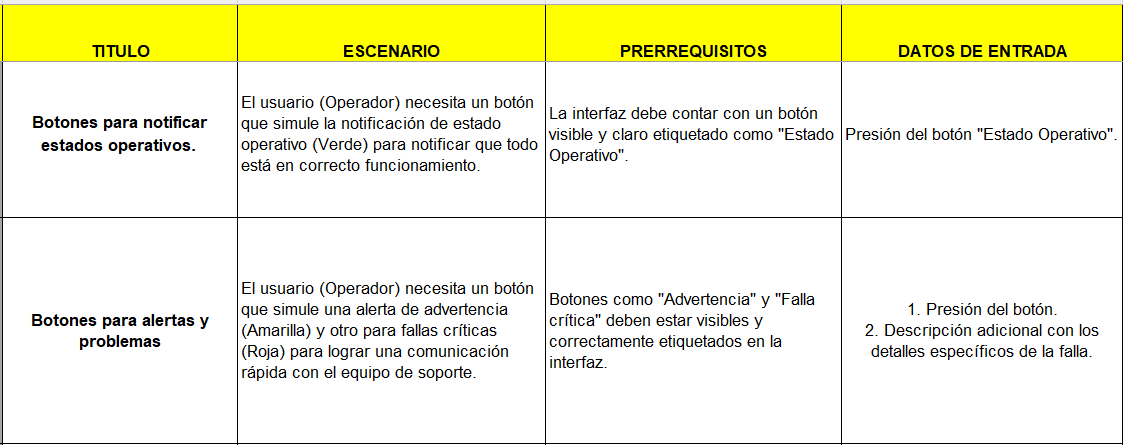
\includegraphics[width=1.0\textwidth]
		{Imagenes/PathAyuda/CPBotonesAndon.png}
		\caption{Caso de Prueba - Simulación de botones - ANDON
		}\label{a2}
	\end{figure}
	
	\begin{figure}[H]
		\centering
		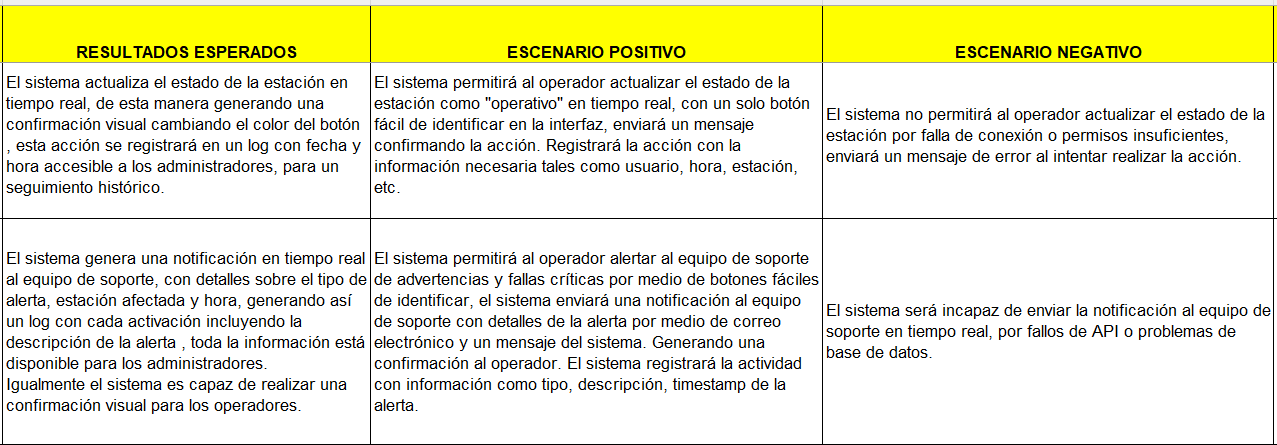
\includegraphics[width=1.0\textwidth]
		{Imagenes/PathAyuda/CPBotonesAndon2.png}
		\caption{Caso de Prueba - Simulación de botones - ANDON
		}\label{a2}
	\end{figure}
	
	\begin{figure}[H]
		\centering
		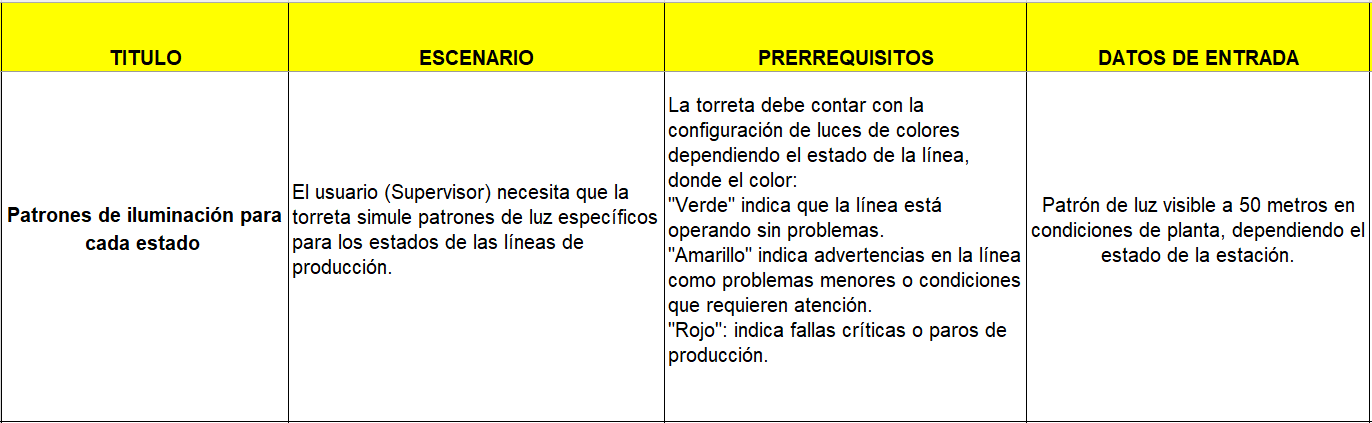
\includegraphics[width=1.0\textwidth]
		{Imagenes/PathAyuda/CPTorreta.png}
		\caption{Caso de Prueba - Configuración y Simulación de Torreta Luminosa
		}\label{a2}
	\end{figure}
	
	\begin{figure}[H]
		\centering
		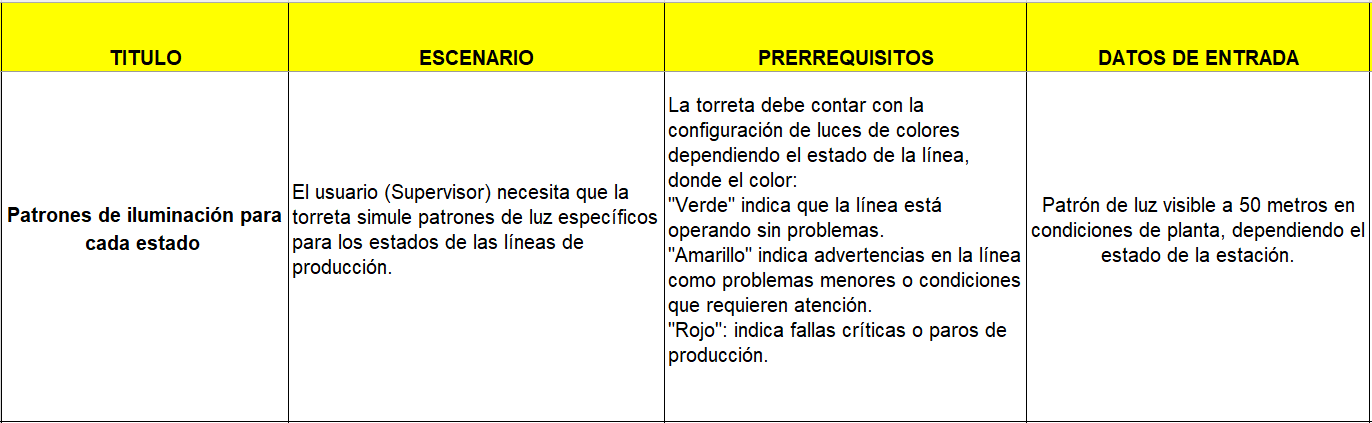
\includegraphics[width=1.0\textwidth]
		{Imagenes/PathAyuda/CPTorreta.png}
		\caption{Caso de Prueba - Configuración y Simulación de Torreta Luminosa
		}\label{a2}
	\end{figure}
	
	\begin{figure}[H]
		\centering
		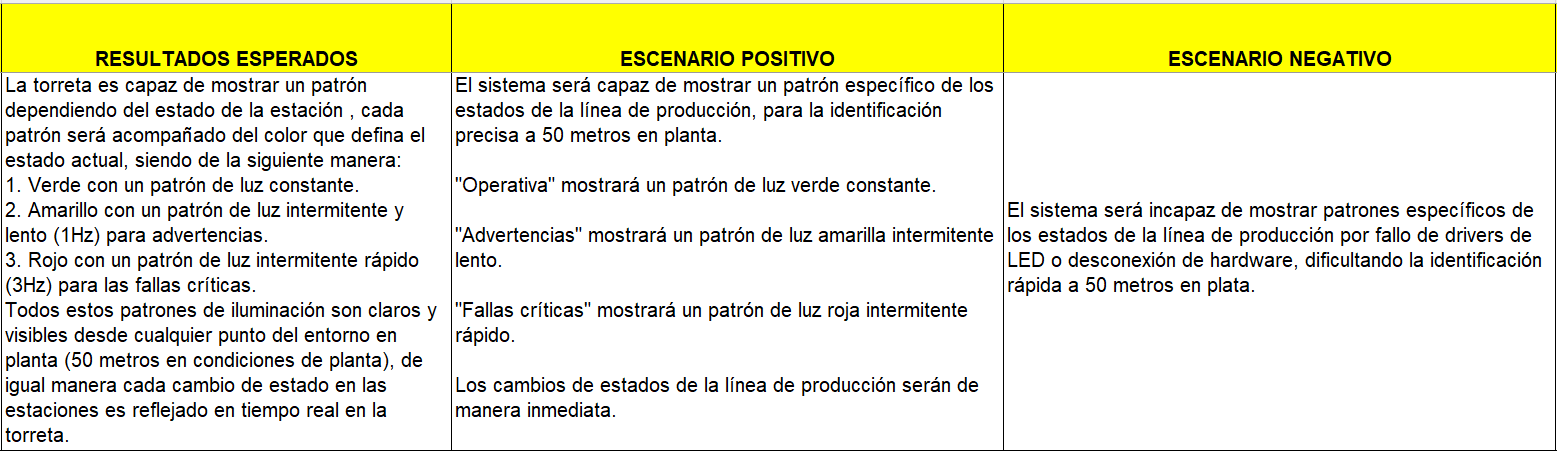
\includegraphics[width=1.0\textwidth]
		{Imagenes/PathAyuda/CPTorreta2.png}
		\caption{Caso de Prueba - Configuración y Simulación de Torreta Luminosa
		}\label{a2}
	\end{figure}
	
	\begin{figure}[H]
		\centering
		\includegraphics[width=1.0\textwidth]
		{Imagenes/PathAyuda/CPMultiCanal.png}
		\caption{Caso de Prueba - Notificaciones Multi-Canal
		}\label{a2}
	\end{figure}
	
	\begin{figure}[H]
		\centering
		\includegraphics[width=1.0\textwidth]
		{Imagenes/PathAyuda/CPMultiCanal2.png}
		\caption{Caso de Prueba - Notificaciones Multi-Canal
		}\label{a2}
	\end{figure}
	
	\begin{figure}[H]
		\centering
		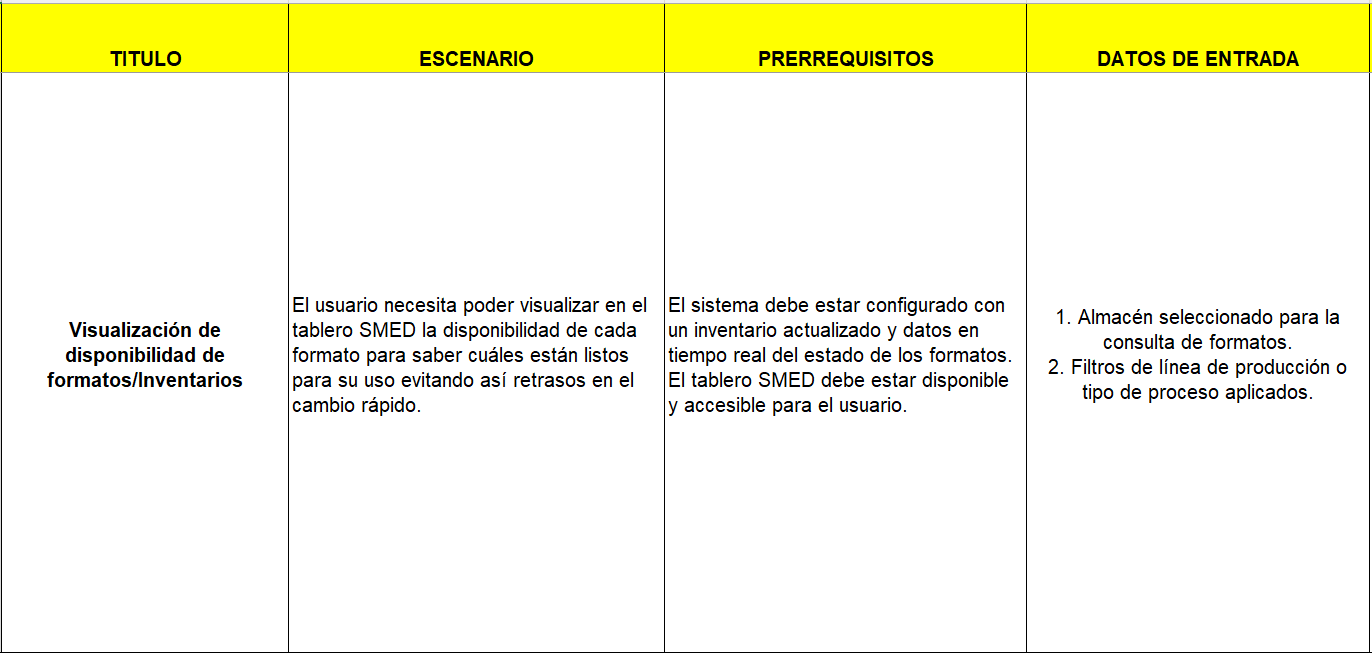
\includegraphics[width=1.0\textwidth]
		{Imagenes/PathAyuda/CPSMED.png}
		\caption{Caso de Prueba - SMED
		}\label{a2}
	\end{figure}
	
	\begin{figure}[H]
		\centering
		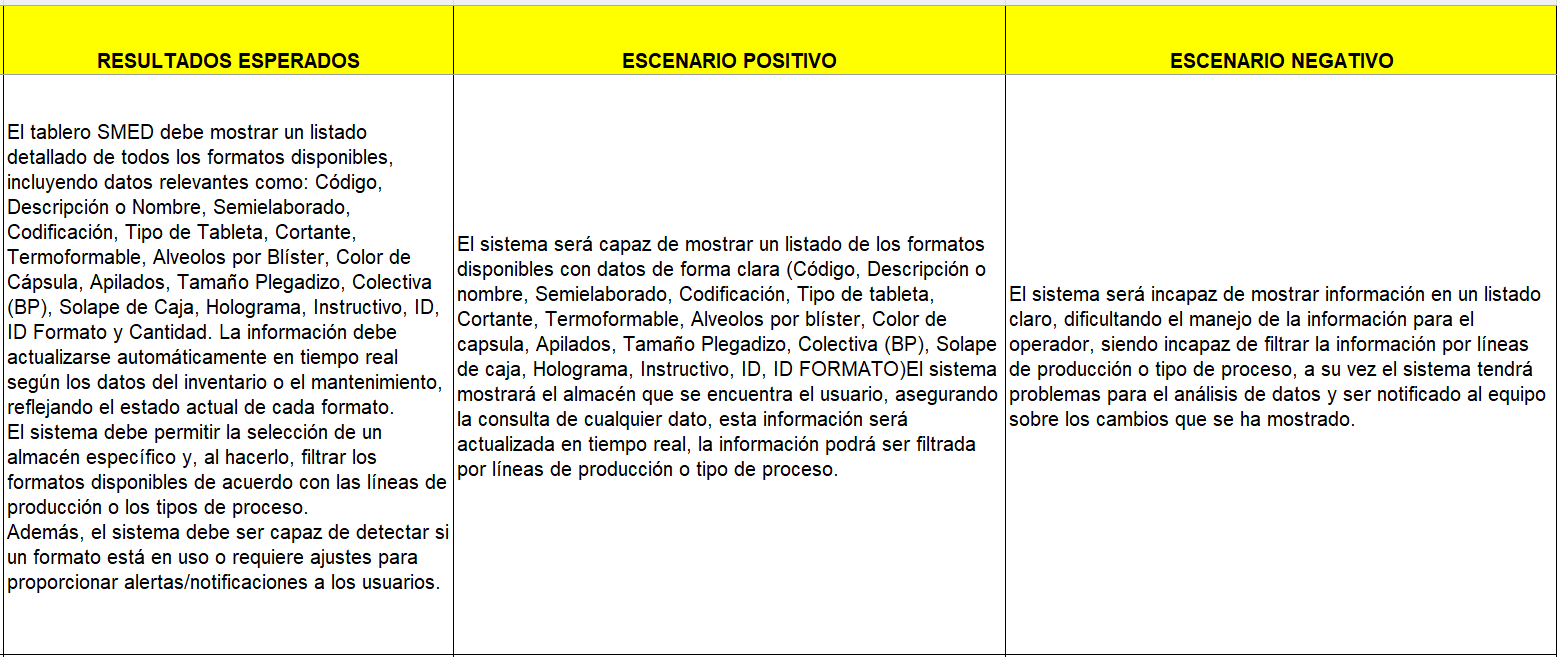
\includegraphics[width=1.0\textwidth]
		{Imagenes/PathAyuda/CPSMED2.png}
		\caption{Caso de Prueba - SMED
		}\label{a2}
	\end{figure}
	
	\begin{figure}[H]
		\centering
		\includegraphics[width=0.9\textwidth]
		{Imagenes/PathAyuda/CPRecetas.png}
		\caption{Caso de Prueba - Gestión de Recetas
		}\label{a2}
	\end{figure}
	
	\begin{figure}[H]
		\centering
		\includegraphics[width=1.0\textwidth]
		{Imagenes/PathAyuda/CPRecetas2.png}
		\caption{Caso de Prueba - Gestión de Recetas
		}\label{a2}
	\end{figure}
	
	\begin{figure}[H]
		\centering
		\includegraphics[width=1.0\textwidth]
		{Imagenes/PathAyuda/CPLineaProduccion.png}
		\caption{Caso de Prueba - Trafico de Líneas de Producción
		}\label{a2}
	\end{figure}
	
	\begin{figure}[H]
		\centering
		\includegraphics[width=1.0\textwidth]
		{Imagenes/PathAyuda/CPLineaProduccion2.png}
		\caption{Caso de Prueba - Trafico de Líneas de Producción
		}\label{a2}
	\end{figure}
	
	\begin{figure}[H]
		\centering
		\includegraphics[width=1.0\textwidth]
		{Imagenes/PathAyuda/CPGestionArea.png}
		\caption{Caso de Prueba - Gestión de Áreas
		}\label{a2}
	\end{figure}
	
	\begin{figure}[H]
		\centering
		\includegraphics[width=1.0\textwidth]
		{Imagenes/PathAyuda/CPGestionArea2.png}
		\caption{Caso de Prueba - Gestión de Áreas
		}\label{a2}
	\end{figure}
	
	\begin{figure}[H]
		\centering
		\includegraphics[width=1.0\textwidth]
		{Imagenes/PathAyuda/CPTask.png}
		\caption{Caso de Prueba - Task Manager (Incidencias ANDON)
		}\label{a2}
	\end{figure}
	
	\begin{figure}[H]
		\centering
		\includegraphics[width=1.0\textwidth]
		{Imagenes/PathAyuda/CPTask2.png}
		\caption{Caso de Prueba - Task Manager (Incidencias ANDON)
		}\label{a2}
	\end{figure}
	
	\newpage
	

\section{Calculadora Nutricional}

	El proyecto Calculadora Nutricional tiene como objetivo modernizar una herramienta desarrollada en 2011 para el cálculo de nutrición parenteral en pacientes adultos, trasladándola a una plataforma web accesible y funcional. La versión original, distribuida en discos físicos y operada mediante un programa instalable, quedó obsoleta con el tiempo, limitando su uso y dificultando la promoción de mezclas individualizadas de SAFE.\\
	
	Para garantizar un desarrollo estructurado y eficiente, se llevó a cabo una documentación completa del proyecto. Este trabajo permitió establecer una base sólida para la planificación y ejecución del desarrollo, asegurando que cada aspecto del sistema estuviera bien definido antes de su implementación.\\
	
	Gracias a esta documentación, se logró una mejor organización del proyecto, facilitando la identificación de necesidades y asegurando que las funcionalidades estuvieran alineadas con los objetivos planteados.Además, permitió estructurar de manera clara las mejoras con respecto a la versión anterior, optimizando el desarrollo y asegurando que la herramienta final sea eficiente, accesible y alineada con las necesidades del sector salud.

\subsection{Levantamiento de requerimientos}

	Para garantizar que la nueva versión de la Calculadora Nutricional cubriera todas las necesidades del personal de salud y mejorara la experiencia del usuario, se llevó a cabo un levantamiento de requerimientos detallado. Durante este proceso, se analizaron tanto las limitaciones de la versión original como las funcionalidades necesarias para optimizar su uso en un entorno web.\\
	
	{\leftskip=1em 
	\noindent 
	\textbf{Usuarios y roles:}\\ 
	Definiendo las diferencias entre usuarios registrados (doctores y personal de salud) y visitantes, estableciendo permisos diferenciados como la capacidad de almacenar y recuperar cálculos.\\
	\par}

	{\leftskip=1em 
	\noindent 
	\textbf{Funcionalidades esenciales:}\\
	Incluyendo el cálculo de mezclas, la impresión de resultados, el almacenamiento en una base de datos y la incorporación de una encuesta inicial para recopilar información de uso.\\
	\par}
	
	{\leftskip=1em 
	\noindent 
	\textbf{Mejoras respecto a la versión anterior:}\\
	Implementando herramientas de monitoreo para conocer quién y desde dónde se utiliza la calculadora, facilitando estrategias de promoción y capacitación.\\
	\par}
	
	{\leftskip=1em 
	\noindent 
	\textbf{Requisitos técnicos y de usabilidad:}\\
	Considerando aspectos como la accesibilidad, la compatibilidad con dispositivos modernos y una interfaz intuitiva.\\
	\par}

\subsection{Casos de prueba}
	
	Para asegurar la fiabilidad de los cálculos y la correcta implementación de las funcionalidades de la Calculadora Nutricional, se diseñó un conjunto de casos de prueba organizados por épicas y centrados en la precisión de las fórmulas médicas, la gestión de usuarios y la usabilidad del sistema.\\

	{\leftskip=1em 
		\noindent 
		\textbf{Escenario:} Situación específica en la que se ejecutará la prueba.
		\par}
	
	{\leftskip=1em 
		\noindent 
		\textbf{Prerrequisitos:} Condiciones que deben cumplirse antes de ejecutar la prueba
		\par}
	
	{\leftskip=1em 
		\noindent 
		\textbf{Datos de Entrada:} Información que se ingresará en el sistema para la ejecución de la prueba.
		\par}
	
	{\leftskip=1em 
		\noindent 
		\textbf{Resultados Esperados:} Comportamiento esperado del sistema tras ejecutar la prueba.
		\par}
	
	{\leftskip=1em 
		\noindent 
		\textbf{Escenarios Positivos:} Pruebas en las que el sistema responde correctamente según lo esperado.
		\par}
	
	{\leftskip=1em 
		\noindent 
		\textbf{Escenarios Negativos:} Pruebas en las que se validan errores o respuestas incorrectas del sistema.\\
		\par}


	Se diseñaron pruebas para garantizar la precisión del sistema, verificando la exactitud de los cálculos, el manejo de errores en los datos de entrada y el acceso adecuado según el tipo de usuario. Además, se validó la correcta generación e impresión de reportes. La documentación detallada de estos casos de prueba permitió establecer un marco sólido para la validación del sistema, asegurando su fiabilidad y facilitando futuras mejoras.\\
	
	
	\begin{figure}[H]
		\centering
		\includegraphics[width=1.0\textwidth]
		{Imagenes/CalculadoraNutricional/CPLogin.png}
		\caption{Caso de Prueba - Log-in
		}\label{a2}
	\end{figure}
	
	\begin{figure}[H]
		\centering
		\includegraphics[width=1.0\textwidth]
		{Imagenes/CalculadoraNutricional/CPLogin2.png}
		\caption{Caso de Prueba - Log-in
		}\label{a2}
	\end{figure}
	
	\begin{figure}[H]
		\centering
		\includegraphics[width=1.0\textwidth]
		{Imagenes/CalculadoraNutricional/CPCuentaMedico.png}
		\caption{Caso de Prueba - Creación de Cuenta para Personal Médico
		}\label{a2}
	\end{figure}
	
	\begin{figure}[H]
		\centering
		\includegraphics[width=1.0\textwidth]
		{Imagenes/CalculadoraNutricional/CPCuentaMedico2.png}
		\caption{Caso de Prueba - Creación de Cuenta para Personal Médico
		}\label{a2}
	\end{figure}
	
	\begin{figure}[H]
		\centering
		\includegraphics[width=1.0\textwidth]
		{Imagenes/CalculadoraNutricional/CPCuentaEstudiante.png}
		\caption{Caso de Prueba - Creación de Cuenta para Personal Médico
		}\label{a2}
	\end{figure}
	
	\begin{figure}[H]
		\centering
		\includegraphics[width=1.0\textwidth]
		{Imagenes/CalculadoraNutricional/CPCuentaEstudiante2.png}
		\caption{Caso de Prueba - Creación de Cuenta para Personal Médico
		}\label{a2}
	\end{figure}
	
	\begin{figure}[H]
		\centering
		\includegraphics[width=1.0\textwidth]
		{Imagenes/CalculadoraNutricional/CPSesionGestion.png}
		\caption{Caso de Prueba - Inicio de Sesión y Gestión de Usuarios
		}\label{a2}
	\end{figure}
	
	\begin{figure}[H]
		\centering
		\includegraphics[width=1.0\textwidth]
		{Imagenes/CalculadoraNutricional/CPSesionGestion2.png}
		\caption{Caso de Prueba - Inicio de Sesión y Gestión de Usuarios
		}\label{a2}
	\end{figure}
	
	
	\begin{figure}[H]
		\centering
		\includegraphics[width=1.0\textwidth]
		{Imagenes/CalculadoraNutricional/CPRolesPermisos.png}
		\caption{Caso de Prueba - Gestión de Roles y Permisos
		}\label{a2}
	\end{figure}
	
	\begin{figure}[H]
		\centering
		\includegraphics[width=1.0\textwidth]
		{Imagenes/CalculadoraNutricional/CPRolesPermisos2.png}
		\caption{Caso de Prueba - Gestión de Roles y Permisos
		}\label{a2}
	\end{figure}
	
	\begin{figure}[H]
		\centering
		\includegraphics[width=1.0\textwidth]
		{Imagenes/CalculadoraNutricional/CPEncuestaEstudiante.png}
		\caption{Caso de Prueba - Encuesta de Registro para Estudiantes y Visitantes
		}\label{a2}
	\end{figure}
	
	\begin{figure}[H]
		\centering
		\includegraphics[width=1.0\textwidth]
		{Imagenes/CalculadoraNutricional/CPEncuestaEstudiante2.png}
		\caption{Caso de Prueba - Encuesta de Registro para Estudiantes y Visitantes
		}\label{a2}
	\end{figure}

	\begin{figure}[H]
		\centering
		\includegraphics[width=1.0\textwidth]
		{Imagenes/CalculadoraNutricional/CPDiseñoInterfaz.png}
		\caption{Caso de Prueba - Diseño de interfaz de Usuario
		}\label{a2}
	\end{figure}
	
	\begin{figure}[H]
		\centering
		\includegraphics[width=1.0\textwidth]
		{Imagenes/CalculadoraNutricional/CPDiseñoInterfaz2.png}
		\caption{Caso de Prueba - Diseño de interfaz de Usuario
		}\label{a2}
	\end{figure}
	
	\begin{figure}[H]
		\centering
		\includegraphics[width=1.0\textwidth]
		{Imagenes/CalculadoraNutricional/CPCalculadora.png}
		\caption{Caso de Prueba - Cálculo de Flujo y Evaluación Nutricional
		}\label{a2}
	\end{figure}
	
	\begin{figure}[H]
		\centering
		\includegraphics[width=1.0\textwidth]
		{Imagenes/CalculadoraNutricional/CPCalculo2.png}
		\caption{Caso de Prueba - Cálculo de Flujo y Evaluación Nutricional
		}\label{a2}
	\end{figure}

	\begin{figure}[H]
		\centering
		\includegraphics[width=1.0\textwidth]
		{Imagenes/CalculadoraNutricional/CPInicio.png}
		\caption{Caso de Prueba - Interfaz de Inicio
		}\label{a2}
	\end{figure}
	
	\begin{figure}[H]
		\centering
		\includegraphics[width=1.0\textwidth]
		{Imagenes/CalculadoraNutricional/CPInicio2.png}
		\caption{Caso de Prueba - Interfaz de Inicio
		}\label{a2}
	\end{figure}
	
	
% CAPITULO RESULTADOS(estatus del proyecto y posibles mejoras) Y CONCLUSIONES(problemas presentados, costos, restrasos, cumplimiento de objetivos, etc)
%____________________________________________________________________________________________________________________
	
	
\chapter{Resultados y Conclusiones}
\newpage
	
\section{Resultados}

\section{Conclusiones}


% -------------------------- ANEXOS
%____________________________________________________________________________________________________________________
	

\newpage
% APENDICE O ANEXO (infoemacion adicional que se quiera anexar o agregar
% BIBLIOGRAFIA
\appendix
	
%\chapter{Bibliograf\check{}�a}
%\bibliographystyle{apalike}
\bibliographystyle{unsrtnat}
	
	




\newpage
\chapter{Bibliografía}

	Sulbarán, I. (2023). \textit{¿Qué es la gestión de proyectos de software? - Tiffin University}. Recuperado 6 de junio de 2023, de https://global.tiffin.edu/blog/en-que-consiste-la-gestion-de-proyectos-de-software:~:text=Alhablardelagestio,alaprcticaseg\\
	
	Gurnov, A. (2023). \textit{¿Qué es la gestión de proyectos de software?}. Recuperado 17 de julio de 2023, de https://www.wrike.com/es/project-management-guide/faq/que-es-la-gestion-de-proyectos-de-software/\\
	
	Arsys. (2024). \textit{Cómo hacer documentación técnica para tu software}. Recuperado en 2024, de https://www.arsys.es/blog/hacer-documentacion-tecnica-software:~:
	text=Laimportancia-de-unadocumentaci,puedevolverseinaccesibleeineficaz\\
	
	IBM. (2024). \textit{Gestión de requisitos. ¿Qué es la gestión de requisitos?}. Recuperado 8 de octubre de 2024, de https://www.ibm.com/mx-es/topics/what-is-requirements-management:~:text\\
	
	Blueoptima\_Admin. (2023). \textit{What Are Function Points in Software Engineering?}. Recuperado 10 de agosto de 2023, de https://www.blueoptima.com/what-are-function-points-in-software-engineering/\\
	
	GeeksforGeeks. (2024). \textit{Functional Point (FP) Analysis Software engineering}. Recuperado 20 de septiembre de 2024, de https://www.geeksforgeeks.org/software-engineering-functional-point-fp-analysis/\\
	
	IBM. (2024, mayo 9). \textit{¿Qué son las pruebas de software y cómo funcionan?} Recuperado de https://www.ibm.com/mx-es/topics/software-testing\\
	
	Roy, S. (2023, junio 21). \textit{Quality Assurance vs Testing}. BrowserStack. Recuperado de https://www.browserstack.com/guide/quality-assurance-vs-testing\\
	
	Schwartz, C. (2025, enero 30). \textit{Test Cases vs Test Scenarios: Definition, Examples and Template}. Leapwork. Recuperado de https://www.leapwork.com/blog/test-case-vs-test-scenario\\
	
	Mapex. (2023, septiembre 15). \textit{Tecnología móvil: ¿cuál es su potencial en las empresas industriales?} Recuperado de https://mapex.io/news/tecnologia-movil-empresas-industriales/\\

\newpage	
\chapter{Glosario}

\begin{description}
	\item[Asesor Acadámico] Persona encargada de regañar a los alumnos
\end{description}
	
%Otro apendice

\end{document} 
